\documentclass[professionalfont, 12pt, dvipdfmx, default, cjk]{beamer}

% the various libraries we will be using
\usepackage{tikz}
\usetikzlibrary{calc}
\usepackage[none]{hyphenat}
\usepackage{longtable}
\usepackage{booktabs}

% macro
\def\BeginColumn#1{\begin{columns}\column{#1\textwidth}}
\def\Column#1{\column{#1\textwidth}}
\def\EndColumn{\end{columns}}
\providecommand{\tightlist}{%
    \setlength{\itemsep}{0pt}\setlength{\parskip}{0pt}}

% define colours
% taken from pickton on Adobe Kuler:
% https://kuler.adobe.com/Some-Kind-Of-Execushares-color-theme-3837185/
\definecolor{ExecusharesRed}{RGB}{230,37,52}
\definecolor{ExecusharesBlack}{RGB}{43,40,40}
\definecolor{ExecusharesBlue}{RGB}{22,190,207}
\definecolor{ExecusharesWhite}{RGB}{255,255,243}
\definecolor{ExecusharesGrey}{RGB}{107,110,108}

% set colours
\setbeamercolor{itemize item}{fg=ExecusharesBlue}
\setbeamercolor{enumerate item}{fg=ExecusharesBlue}
\setbeamercolor{alerted text}{fg=ExecusharesBlue}
\setbeamercolor{section in toc}{fg=ExecusharesBlack}

% set fonts
\setbeamerfont{itemize/enumerate body}{size=\large}
\setbeamerfont{itemize/enumerate subbody}{size=\normalsize}
\setbeamerfont{itemize/enumerate subsubbody}{size=\small}

% make the itemize bullets pixelated >
\setbeamertemplate{itemize item}{
  \tikz{
    \draw[fill=ExecusharesBlue,draw=none] (0, 0) rectangle(0.1, 0.1);
    \draw[fill=ExecusharesBlue,draw=none] (0.1, 0.1) rectangle(0.2, 0.2);
    \draw[fill=ExecusharesBlue,draw=none] (0, 0.2) rectangle(0.1, 0.3);
  }
}
% make the subitems also pixelated >, but a little smaller and red
\setbeamertemplate{itemize subitem}{
  \tikz{
    \draw[fill=ExecusharesRed,draw=none] (0, 0) rectangle(0.075, 0.075);
    \draw[fill=ExecusharesRed,draw=none] (0.075, 0.075) rectangle(0.15, 0.15);
    \draw[fill=ExecusharesRed,draw=none] (0, 0.15) rectangle(0.075, 0.225);
  }
}

% disable navigation
\setbeamertemplate{navigation symbols}{}

% custom draw the title page above
\setbeamertemplate{title page}{}

% again, manually draw the frame title above
\setbeamertemplate{frametitle}{}

% disable "Figure:" in the captions
\setbeamertemplate{caption}{\tiny\insertcaption}
\setbeamertemplate{caption label separator}{}

% since I don't know a better way to do this, these are all switches
% doing `\setcounter{showProgressBar}{0}` will turn the progress bar off (I turn it off for Appendix slides)
% etc
\newcounter{showProgressBar}
\setcounter{showProgressBar}{1}
\newcounter{showSlideNumbers}
\setcounter{showSlideNumbers}{1}
\newcounter{showSlideTotal}
\setcounter{showSlideTotal}{1}

% use \makeatletter for our progress bar definitions
% progress bar idea from http://tex.stackexchange.com/a/59749/44221
% slightly adapted for visual purposes here
\makeatletter
\newcount\progressbar@tmpcounta% auxiliary counter
\newcount\progressbar@tmpcountb% auxiliary counter
\newdimen\progressbar@pbwidth %progressbar width
\newdimen\progressbar@tmpdim % auxiliary dimension

\newdimen\slidewidth % auxiliary dimension
\newdimen\slideheight % auxiliary dimension

% make the progress bar go across the screen
%\progressbar@pbwidth=12.8cm
\progressbar@pbwidth=\the\paperwidth
\slidewidth=\the\paperwidth
\slideheight=\the\paperheight

% use tikz to draw everything
% it may not be the best, but it's easy to work with
% and looks good
% TODO: base title slide and contents slide on something other than slide numbers :/
\setbeamertemplate{background}{
  % deal with progress bar stuff
  % (calculate where it should go)
  \progressbar@tmpcounta=\insertframenumber
  \progressbar@tmpcountb=\inserttotalframenumber
  % \advance\progressbar@tmpcounta by -1
  % \advance\progressbar@tmpcountb by -1
  \progressbar@tmpdim=\progressbar@pbwidth
  \multiply\progressbar@tmpdim by \progressbar@tmpcounta
  \divide\progressbar@tmpdim by \progressbar@tmpcountb

  
\begin{tikzpicture}
    % set up the entire slide as the canvas
    \useasboundingbox (0,0) rectangle(\the\paperwidth,\the\paperheight);

    % the background
    \fill[color=ExecusharesWhite] (0,0) rectangle(\the\paperwidth,\the\paperheight);

    % separate the drawing based on if we're the first (title) slide or not
    \ifnum\thepage=1\relax
      % the title page
      % draw the fills
      \fill[color=ExecusharesRed] (0, 4cm) rectangle(\slidewidth,\slideheight);

      % draw the actual text
      \node[anchor=south,text width=\slidewidth-1cm,inner xsep=0.5cm] at (0.5\slidewidth,4cm) {\color{ExecusharesWhite}\Huge\textbf{\inserttitle}};
      \node[anchor=north east,text width=\slidewidth-1cm,align=right] at (\slidewidth-0.4cm,4cm) {\color{ExecusharesBlack}\tiny\insertsubtitle};
      \node[above] at(0.5\slidewidth,2.3cm) {\color{ExecusharesBlack}\tiny by};
      \node at (0.5\slidewidth,2cm) {\color{ExecusharesBlack}\LARGE\insertauthor};

      % add the date in the corner
      \node[anchor=south east] at(\slidewidth,0cm) {\color{ExecusharesGrey}\tiny\insertdate};
    \else
      % NOT the title page
      % title bar
      \fill[color=ExecusharesRed] (0, \slideheight-1cm) rectangle(\slidewidth,\slideheight);

      % swap the comment on these to add section titles to slide titles
      %\node[anchor=north,text width=11.8cm,inner xsep=0.5cm,inner ysep=0.25cm] at (6.4cm,9.6cm) {\color{ExecusharesWhite}\Large\textbf{\insertsectionhead: \insertframetitle}};
      \node[anchor=north,text width=\slidewidth-1cm,inner xsep=0.5cm,inner ysep=0.25cm] at (0.5\slidewidth,\slideheight) {\color{ExecusharesWhite}\huge\textbf{\insertframetitle}};
      
      % if we're showing a progress bar, show it
      % (I disable the progress bar and slide numbers for the "Appendix" slides)
      \ifnum \value{showProgressBar}>0\relax%
        % the the progress bar icon in the middle of the screen
        \draw[fill=ExecusharesGrey,draw=none] (0cm,0cm) rectangle(\slidewidth,0.25cm);
        \draw[fill=ExecusharesRed,draw=none] (0cm,0cm) rectangle(\progressbar@tmpdim,0.25cm);

        % bottom information
        \node[anchor=south west] at(0cm,0.25cm) {\color{ExecusharesGrey}\tiny\insertsection};
        % if slide numbers are active
        \ifnum \value{showSlideNumbers}>0\relax%
          % if slide totals are active
          \ifnum \value{showSlideTotal}>0\relax%
            % draw both slide number and slide total
            \node[anchor=south east] at(\slidewidth,0.25cm) {\color{ExecusharesGrey}\tiny\insertframenumber/\inserttotalframenumber};
          \else
            % slide totals aren't active, don't draw them
            \node[anchor=south east] at(\slidewidth,0.25cm) {\color{ExecusharesGrey}\tiny\insertframenumber};
          \fi
        \fi
      % don't show the progress bar?
      \else
        % section title in the bottom left
        \node[anchor=south west] at(0cm,0cm) {\color{ExecusharesGrey}\tiny\insertsection};
        % if we're showing slide numbers
        \ifnum \value{showSlideNumbers}>0\relax%
          % if slide totals are active
          \ifnum \value{showSlideTotal}>0\relax%
            % draw both slide number and slide total
            \node[anchor=south east] at(\slidewidth,0cm) {\color{ExecusharesGrey}\tiny\insertframenumber/\inserttotalframenumber};
          \else
            % slide totals aren't active, don't draw them
            \node[anchor=south east] at(\slidewidth,0cm) {\color{ExecusharesGrey}\tiny\insertframenumber};
          \fi
        \fi
      \fi
    \fi
  \end{tikzpicture}
}
\makeatother

% add section titles
\AtBeginSection{\frame{\sectionpage}}
\setbeamertemplate{section page}
{
  
\begin{tikzpicture}
    % set up the entire slide as the canvas
    \useasboundingbox (0,0) rectangle(\slidewidth,\slideheight);
    %\fill[color=ExecusharesWhite] (0,0) rectangle(\the\paperwidth,\the\paperheight);
    \fill[color=ExecusharesWhite] (-1cm, 2cm) rectangle (\slidewidth, \slideheight+0.1cm);
    \fill[color=ExecusharesRed] (-1cm, 0.5\slideheight-1cm) rectangle(\slidewidth, 0.5\slideheight+1cm);
    \node[text width=\the\paperwidth-1cm,align=center] at (0.4\slidewidth, 0.5\slideheight) {\color{ExecusharesWhite}\Huge\textbf{\insertsection}};
  \end{tikzpicture}
}

% source code syntax highlight

\title{Alba Marina Málaga Sabogal}
\author{Candidature au poste de maître de conférences n°1320}
\date{
\includegraphics[width=\textwidth,height=0.5in]{logo_loria_complet.jpg}
\includegraphics[width=\textwidth,height=0.5in]{logo_iutsd.jpg}
\includegraphics[width=\textwidth,height=0.5in]{logo_ul.jpg}}

\begin{document}
\frame{\titlepage}
\hypertarget{parcours}{%
\section{Parcours}\label{parcours}}

\begin{frame}{Enseignement, recherche, développement, médiation}
\protect\hypertarget{enseignement-recherche-duxe9veloppement-muxe9diation}{}
\centering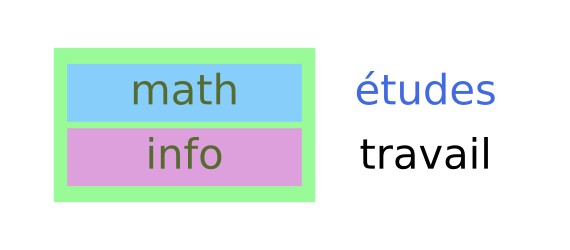
\includegraphics[width=0.25\textwidth,height=\textheight]{timeline_legende.png}

\par

\centering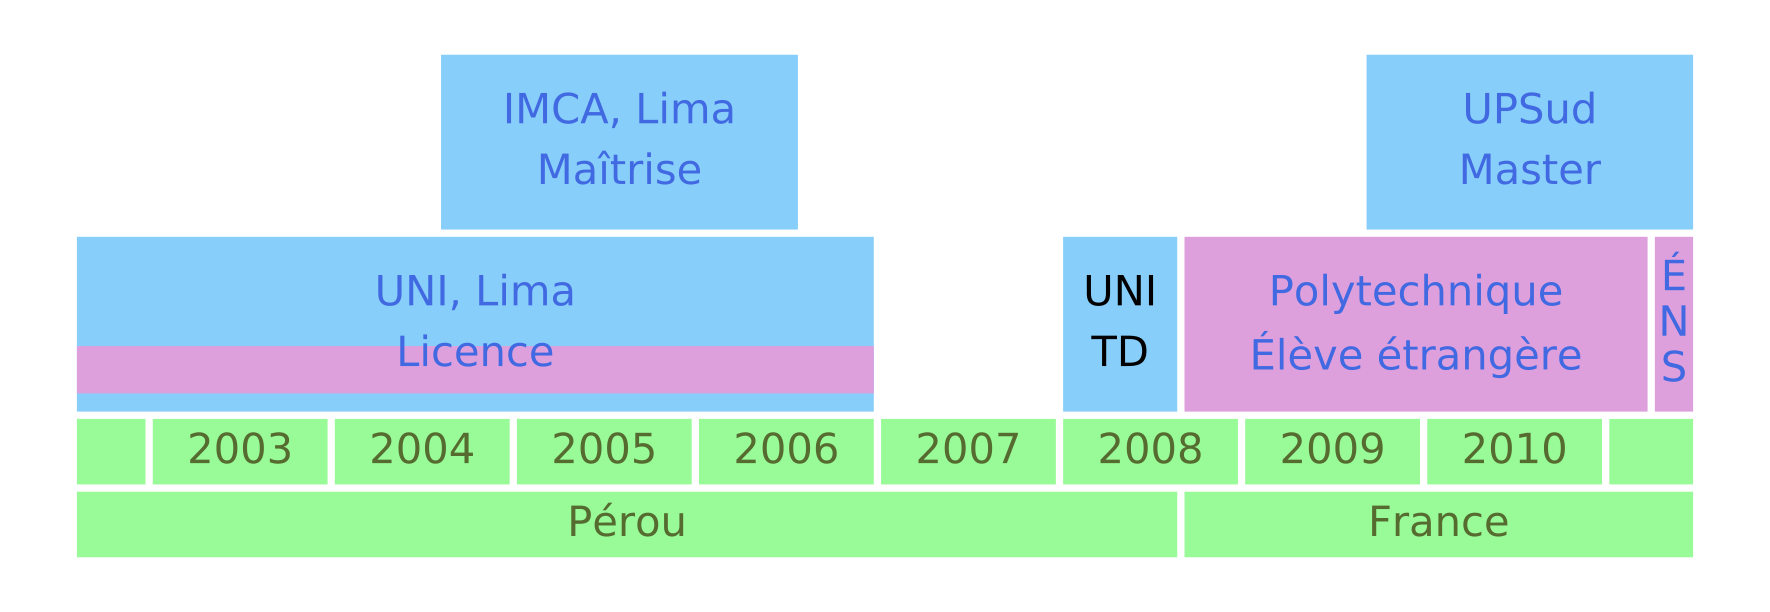
\includegraphics[width=0.9\textwidth,height=\textheight]{alba-timeline-etudes.png}

\par

\centering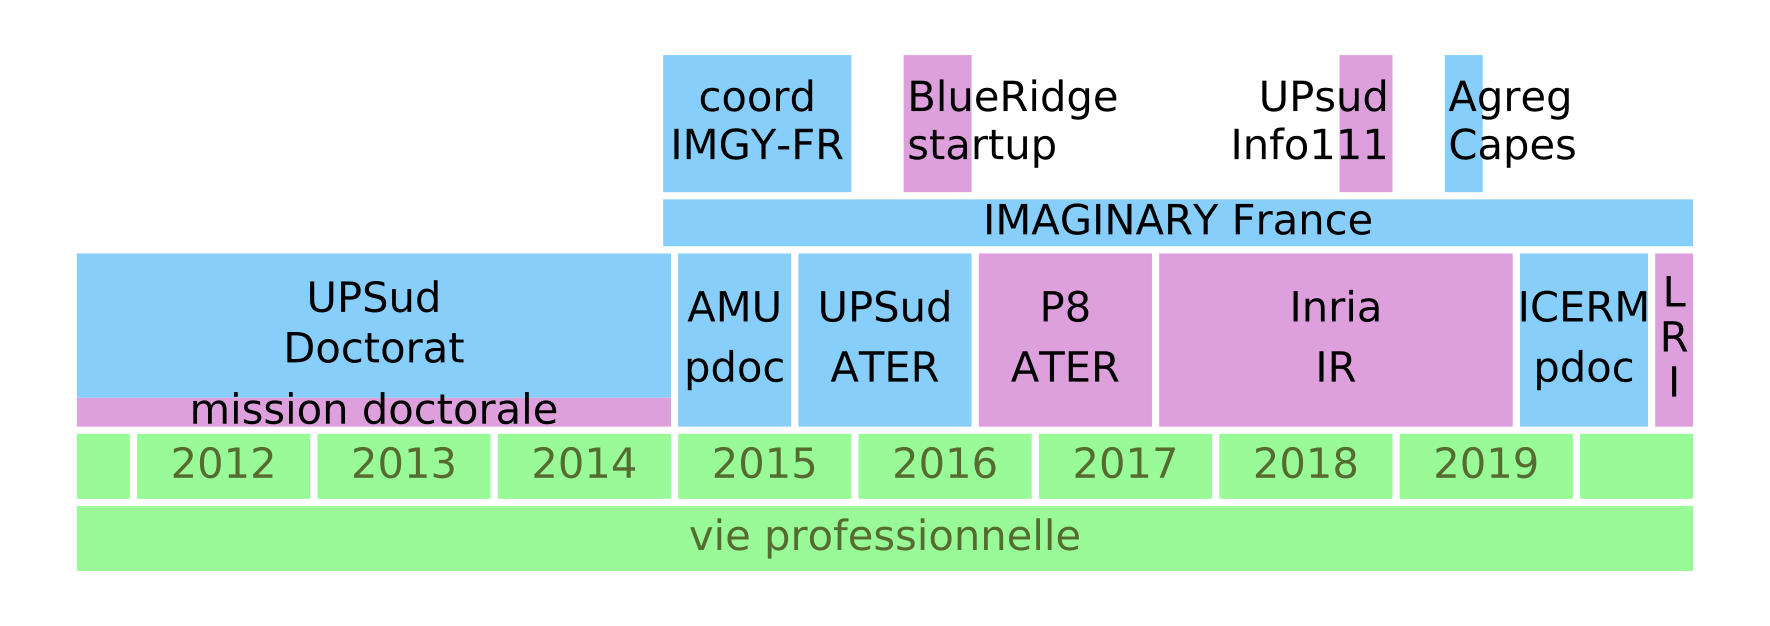
\includegraphics[width=0.9\textwidth,height=\textheight]{alba-timeline-viepro.png}

\par
\end{frame}

\hypertarget{enseignement}{%
\section{Enseignement}\label{enseignement}}

\begin{frame}{Expériences d'enseignement}
\protect\hypertarget{expuxe9riences-denseignement}{}
\begin{longtable}[]{@{}rlr@{}}
\toprule
\endhead
2018 & U Paris-Sud (60h) & CEV Informatique\tabularnewline
& & L1, TD/TP\tabularnewline
& & C++, Jupyter\tabularnewline
& &\tabularnewline
2016--2017 & U Paris 8 (192h) & ATER Informatique\tabularnewline
& & L2, M1, accessibilité\tabularnewline
& & Wordpress, Python\tabularnewline
& &\tabularnewline
2015--2016 & U Paris-Sud (192h) &\tabularnewline
2014 & U Paris-Sud (96h) &\tabularnewline
2008 & UNI (192h) &\tabularnewline
\bottomrule
\end{longtable}

Au total, \(>\) \textbf{600 h} dont \textbf{192h} responsable de cours.
\end{frame}

\begin{frame}{Cours donnés :}
\protect\hypertarget{cours-donnuxe9s}{}
En L1 MPI (chargée de TD/TP) : Intro. à l'informatique (C++)

En L2 MIASHS Accessibilité/Géographie/Langage:

\begin{itemize}
\tightlist
\item
  Calcul formel

  \begin{itemize}
  \tightlist
  \item
    SageMath, pour lequel il faut apprendre le Python
  \end{itemize}
\item
  Mathématiques numériques :

  \begin{itemize}
  \tightlist
  \item
    langage Python - calcul scientifique avec numpy/scipy
  \end{itemize}
\end{itemize}

En M1 MIASHS Accessibilité/Géomatique:

\begin{itemize}
\tightlist
\item
  Programmation objet 1 et 2

  \begin{itemize}
  \tightlist
  \item
    Java pour un public majoritairement neoinformaticien
  \end{itemize}
\item
  \textbf{CMS} et frameworks accessibles

  \begin{itemize}
  \tightlist
  \item
    Wordpress, y compris developpement de thèmes/plugins
  \end{itemize}
\end{itemize}

Mais aussi: TD de géométrie et analyse en PCSO et d'autres cours de
mathématiques
\end{frame}

\begin{frame}{Mon ATER à l'Université Paris 8 Vincennes Saint-Denis:}
\protect\hypertarget{mon-ater-uxe0-luniversituxe9-paris-8-vincennes-saint-denis}{}
\centering
\includegraphics[width=0.15\textwidth,height=\textheight]{logop8-2.png}

\par

Charge de travail équivalente déjà à un MCF :

\begin{itemize}
\tightlist
\item
  seule personne à charge de tous mes cours
\item
  préparation de deux cours pour une nouvelle formation (la licence
  MIASHS)
\item
  encadrement d'un étudiant de géomatique en alternance
\end{itemize}

L'accessibilité :

\begin{itemize}
\tightlist
\item
  thème principal du labo THIM, des formations MIASHS
\item
  des étudiants aveugles en master

  \begin{itemize}
  \tightlist
  \item
    j'ai dû revoir de fond en comble ma façon d'enseigner
  \end{itemize}
\end{itemize}
\end{frame}

\begin{frame}{Le PPN du DUT MMI}
\protect\hypertarget{le-ppn-du-dut-mmi}{}
Dans l'organisation actuelle : 5 catégories, 2 UE par semestre, un
enseignement progressif à partir des bases.

\begin{longtable}[]{@{}lll@{}}
\toprule
\begin{minipage}[b]{0.30\columnwidth}\raggedright
Unités d'enseignement\strut
\end{minipage} & \begin{minipage}[b]{0.27\columnwidth}\raggedright
Catégories\strut
\end{minipage} & \begin{minipage}[b]{0.35\columnwidth}\raggedright
Progression\strut
\end{minipage}\tabularnewline
\midrule
\endhead
\begin{minipage}[t]{0.30\columnwidth}\raggedright
Communication, culture et connaissance de l'environnement
socio-économique\strut
\end{minipage} & \begin{minipage}[t]{0.27\columnwidth}\raggedright
Com./écriture\strut
\end{minipage} & \begin{minipage}[t]{0.35\columnwidth}\raggedright
bases\strut
\end{minipage}\tabularnewline
\begin{minipage}[t]{0.30\columnwidth}\raggedright
\strut
\end{minipage} & \begin{minipage}[t]{0.27\columnwidth}\raggedright
Esth./vidéo\strut
\end{minipage} & \begin{minipage}[t]{0.35\columnwidth}\raggedright
approfondissement\strut
\end{minipage}\tabularnewline
\begin{minipage}[t]{0.30\columnwidth}\raggedright
\textbf{\emph{Culture technologique et développement multimédia}}\strut
\end{minipage} & \begin{minipage}[t]{0.27\columnwidth}\raggedright
\textbf{\emph{Info./réseaux}}\strut
\end{minipage} & \begin{minipage}[t]{0.35\columnwidth}\raggedright
maîtrise\strut
\end{minipage}\tabularnewline
\begin{minipage}[t]{0.30\columnwidth}\raggedright
\strut
\end{minipage} & \begin{minipage}[t]{0.27\columnwidth}\raggedright
\emph{Transversal}\strut
\end{minipage} & \begin{minipage}[t]{0.35\columnwidth}\raggedright
\strut
\end{minipage}\tabularnewline
\begin{minipage}[t]{0.30\columnwidth}\raggedright
\strut
\end{minipage} & \begin{minipage}[t]{0.27\columnwidth}\raggedright
Professionnalisation\strut
\end{minipage} & \begin{minipage}[t]{0.35\columnwidth}\raggedright
approche professionalisante\strut
\end{minipage}\tabularnewline
\bottomrule
\end{longtable}
\end{frame}

\begin{frame}{Cours de la catégorie informatique / réseaux}
\protect\hypertarget{cours-de-la-catuxe9gorie-informatique-ruxe9seaux}{}
\begin{longtable}[]{@{}cl@{}}
\toprule
\endhead
M1202 & Algorithmique et programmation\tabularnewline
M1203 & Services sur réseaux\tabularnewline
M1205 & Intégration web\tabularnewline
M2203 & Base de données\tabularnewline
M2204 & Services sur réseaux 2\tabularnewline
M2206 & Intégration web\tabularnewline
M3202 & Développement web\tabularnewline
M3203 & Programmation objet et événementielle\tabularnewline
M3204 & Services sur réseaux 3\tabularnewline
M3206 & Intégration multimédia\tabularnewline
M4201C & Développement multimédia\tabularnewline
M4203C & Intégration gestion de contenu\tabularnewline
\bottomrule
\end{longtable}
\end{frame}

\begin{frame}
\centering
\includegraphics[width=1\textwidth,height=\textheight]{cours-info-reseaux.png}

\par
\end{frame}

\begin{frame}
\centering
\includegraphics[width=1\textwidth,height=\textheight]{cours-info-reseaux-vert-1.png}

\par
\end{frame}

\begin{frame}
\centering
\includegraphics[width=1\textwidth,height=\textheight]{cours-info-reseaux-vert-2.png}

\par
\end{frame}

\begin{frame}
\centering
\includegraphics[width=1\textwidth,height=\textheight]{cours-info-reseaux-jaune.png}

\par
\end{frame}

\begin{frame}
\centering
\includegraphics[width=1\textwidth,height=\textheight]{cours-info-reseaux-orange.png}

\par
\end{frame}

\begin{frame}{Cours d'autres catégories}
\protect\hypertarget{cours-dautres-catuxe9gories}{}
La catégorie esthétique/vidéo:

\begin{itemize}
\tightlist
\item
  pas du domaine des MCF27 en général mais j'y vois l'opportunité pour
  des intéractions enrichissantes
\item
  j'ai déjà scripté la création de fichiers svg en SageMath/Python et je
  produis dès fichiers pour l'impression 3D avec Blender
\item
  je pourrais peut-être faire une intervention ? un atelier conjoint ?
\end{itemize}

La catégorie transversale:

Culture scientifique et traitement de l'information - cours de
mathématiques sur trois semestres.

\centering
\includegraphics[width=0.05\textwidth,height=\textheight]{vert.png}
Je suis prête à l'enseigner dès demain.

\includegraphics[width=0.05\textwidth,height=\textheight]{vert.png}

\par

\textbf{Les licences pro Cross Media et TeCAM}: \ldots{} plein de
possibilités.
\end{frame}

\begin{frame}{Contribuer une pierre au PPP}
\protect\hypertarget{contribuer-une-pierre-au-ppp}{}
\centering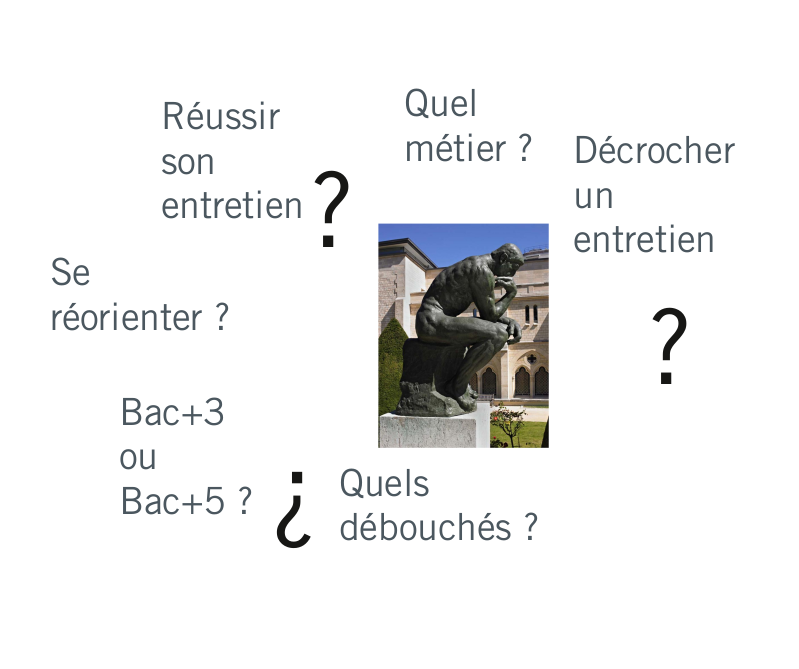
\includegraphics[width=0.7\textwidth,height=\textheight]{ppp-penseur-rodin.png}

\par

Mon réseau: Meetups, AudiMath, Conférences, Tiers lieux, Séminaires,
IMAGINARY
\end{frame}

\begin{frame}{Projets tutorés à l'international}
\protect\hypertarget{projets-tutoruxe9s-uxe0-linternational}{}
\centering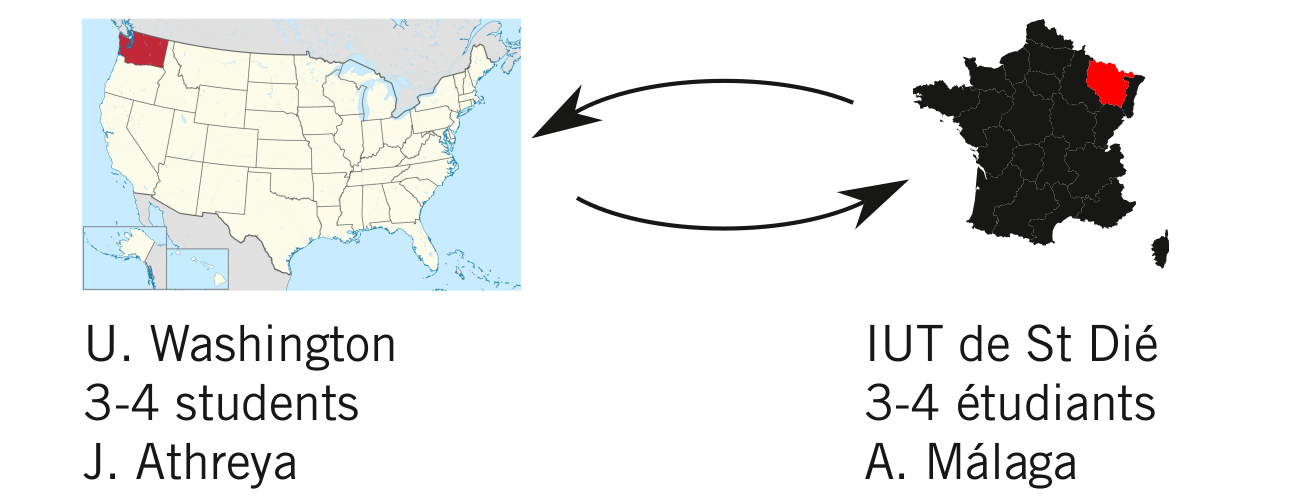
\includegraphics[width=1\textwidth,height=\textheight]{carte-washington-st-die-avec-noms.png}

\par

Exemples de projets :

\begin{itemize}
\tightlist
\item
  explorations de formes fractales
\item
  les mathématiques des épidemies
\item
  les grandes migrations
\end{itemize}
\end{frame}

\begin{frame}{Autre proposition de projet tutoré}
\protect\hypertarget{autre-proposition-de-projet-tutoruxe9}{}
Conception de casse-têtes en impression 3D et découpe laser

\begin{itemize}
\tightlist
\item
  regarder des casse-têtes existants (mathématiques ou pas)
\item
  leur chercher d'autres expressions
\item
  s'en inspirer pour d'autres casse-têtes
\item
  venir les presenter en salon
\end{itemize}

\centering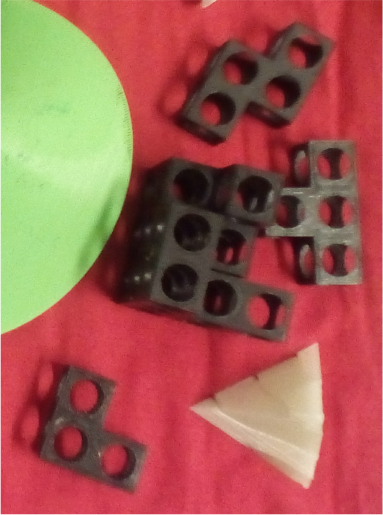
\includegraphics{casse-tetes-3d.png}

\par
\end{frame}

\begin{frame}{La médiation scientifique}
\protect\hypertarget{la-muxe9diation-scientifique}{}
médiation autour de projets d'Art-Science dans le cadre de mon contrat
doctoral : •« La lumière ne s'arrête pas là »•« Premières intimités de
l'être »•« Turbulent »•

\centering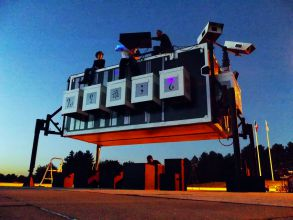
\includegraphics[width=0.4\textwidth,height=\textheight]{../scribus/img/sl_crbst_02-poly-nuit-300dp-l15cm__20.jpg}

\par

\begin{itemize}
\tightlist
\item
  IMAGINARY France

  \begin{itemize}
  \tightlist
  \item
    plus de 150 heures face au grand public
  \item
    plus de 10 événements organisés ; une rencontre autour des
    plateformes de partage
  \item
    résautage actif : incitation à de nouvelles contributions, gestion
    des bénévoles
  \end{itemize}
\end{itemize}

\(+\) les sorties en école, forums, etc. avec les collègues
\end{frame}

\begin{frame}{Intégration au MMI}
\protect\hypertarget{intuxe9gration-au-mmi}{}
\begin{itemize}
\tightlist
\item
  compétence pour enseigner les cours techniques
\item
  intérêt pour la médiation et donc la communication
\item
  souci de l'accessibilité
\end{itemize}

\centering
\includegraphics[width=0.15\textwidth,height=\textheight]{logoMMI.png}

\par
\end{frame}

\hypertarget{recherche}{%
\section{Recherche}\label{recherche}}

\begin{frame}{Les systèmes dynamiques}
\protect\hypertarget{les-systuxe8mes-dynamiques}{}
\begin{itemize}
\tightlist
\item
  Evolution deterministe à court terme, qu'on connaît.
\item
  Les questions qu'on se pose concernent l'évolution à long terme.
\end{itemize}
\end{frame}

\begin{frame}{Un exemple concret : les rotations du cercle:}
\protect\hypertarget{un-exemple-concret-les-rotations-du-cercle}{}
\(α\) nombre\\
\(ρ:𝕊^1\to 𝕊^1\) rotation par un angle \(α\)\\


\includegraphics[width=\textwidth,height=3.125in]{cercle-arc.png}

Conjugué à :


\includegraphics{segment-segment.png}

\(𝕋 = ℝ/ℤ = [0,1]/\{0\sim 1\}\).
\end{frame}

\begin{frame}{Les rotations comme échanges d'intervalles}
\protect\hypertarget{les-rotations-comme-uxe9changes-dintervalles}{}
Paramétre: \(α ∈ [0,1[\)\\
Espace des phases: \(𝕋 = ℝ/ℤ = [0,1]/\{0\sim 1\}\)\\

\(\begin{array}{rcrcl} ρ_- & : & [0,1-α[ & \to & [α,1[\\  & & x & \mapsto & x + α \end{array}\)

\(\begin{array}{rcrcl} ρ_+ & : & [1-α,1[ & \to & [0,α[\\  & & x & \mapsto & x + α - 1 \end{array}\)
\end{frame}

\begin{frame}{Un exemple fondamental: le tore}
\protect\hypertarget{un-exemple-fondamental-le-tore}{}
\href{http://albamath.com/snake}{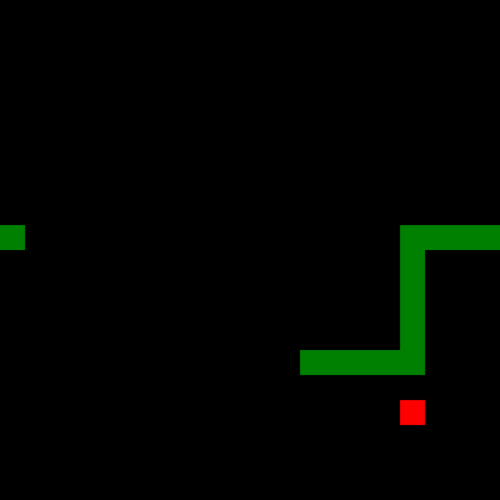
\includegraphics{snake-on-a-torus.png}}
\end{frame}

\begin{frame}{La caracteristique d'Euler et le genre:}
\protect\hypertarget{la-caracteristique-deuler-et-le-genre}{}
\href{http://albamath.com/snake}{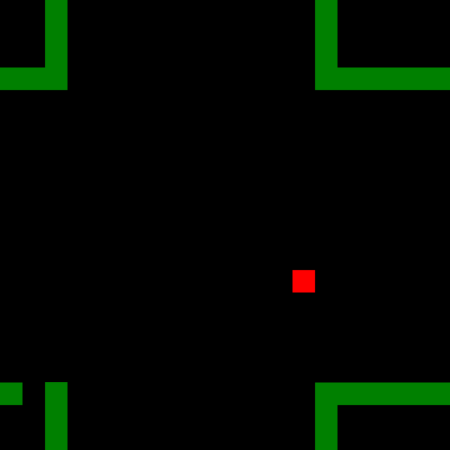
\includegraphics{snake-around-corners.png}}

\(χ = V-E+F = 1 - 2 + 1 = 0\)\\
\(χ=2-2g\)\\
\(g=1\)
\end{frame}

\begin{frame}{Un autre exemple simple de surface de translation: le L}
\protect\hypertarget{un-autre-exemple-simple-de-surface-de-translation-le-l}{}
\href{http://albamath.com/snake-L}{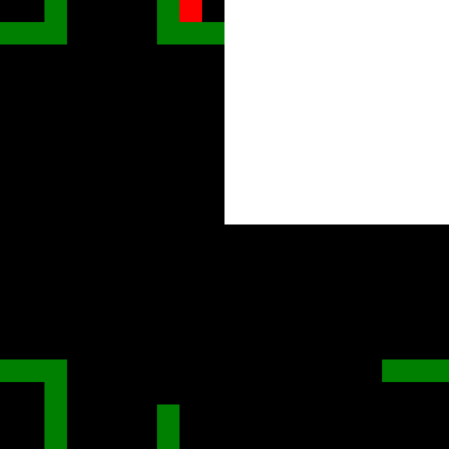
\includegraphics{snake-l-corner.png}}
\end{frame}

\begin{frame}{La caracteristique d'Euler et le genre du L:}
\protect\hypertarget{la-caracteristique-deuler-et-le-genre-du-l}{}
\href{http://albamath.com/snake-L}{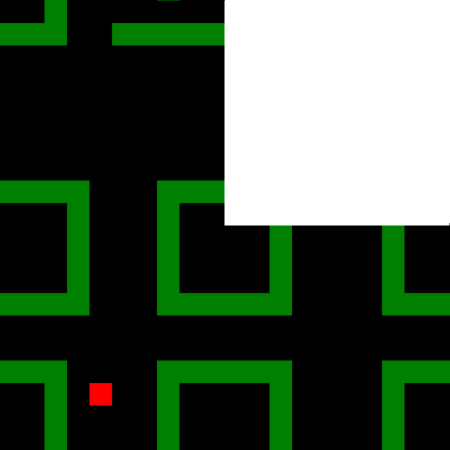
\includegraphics{snake-l-corner-4.png}}

\(χ = V-E+F = 1 - 6 + 3 = -2\)\\
\(χ=2-2g\)\\
\(g=2\)
\end{frame}

\begin{frame}{Une autre vue du L:}
\protect\hypertarget{une-autre-vue-du-l}{}
\href{http://albamath.com/snakeX}{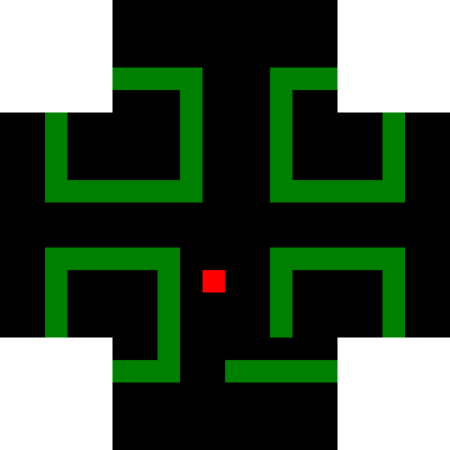
\includegraphics{snake-x-corner-4.png}}

\(χ = V-E+F = 1 - 6 + 3 = -2\)\\
\(χ=2-2g\)\\
\(g=2\)
\end{frame}

\begin{frame}{Définition de surface de translation ``finie''.}
\protect\hypertarget{duxe9finition-de-surface-de-translation-finie.}{}
Une surface de translation est une surface compacte sans bord qui,
privée d'un nombre fini de points, possède un atlas tel que que les
changements de cartes dans cet atlas sont des translations. Supposons
que l'atlas est maximal - les points non couverts par l'atlas sont des
singularités coniques de la géométrie de la surface avec un angle qui
est un multiple entier de 360 degrés.
\end{frame}

\begin{frame}{Dynamique sur une surface de translation}
\protect\hypertarget{dynamique-sur-une-surface-de-translation}{}
\begin{figure}
\centering
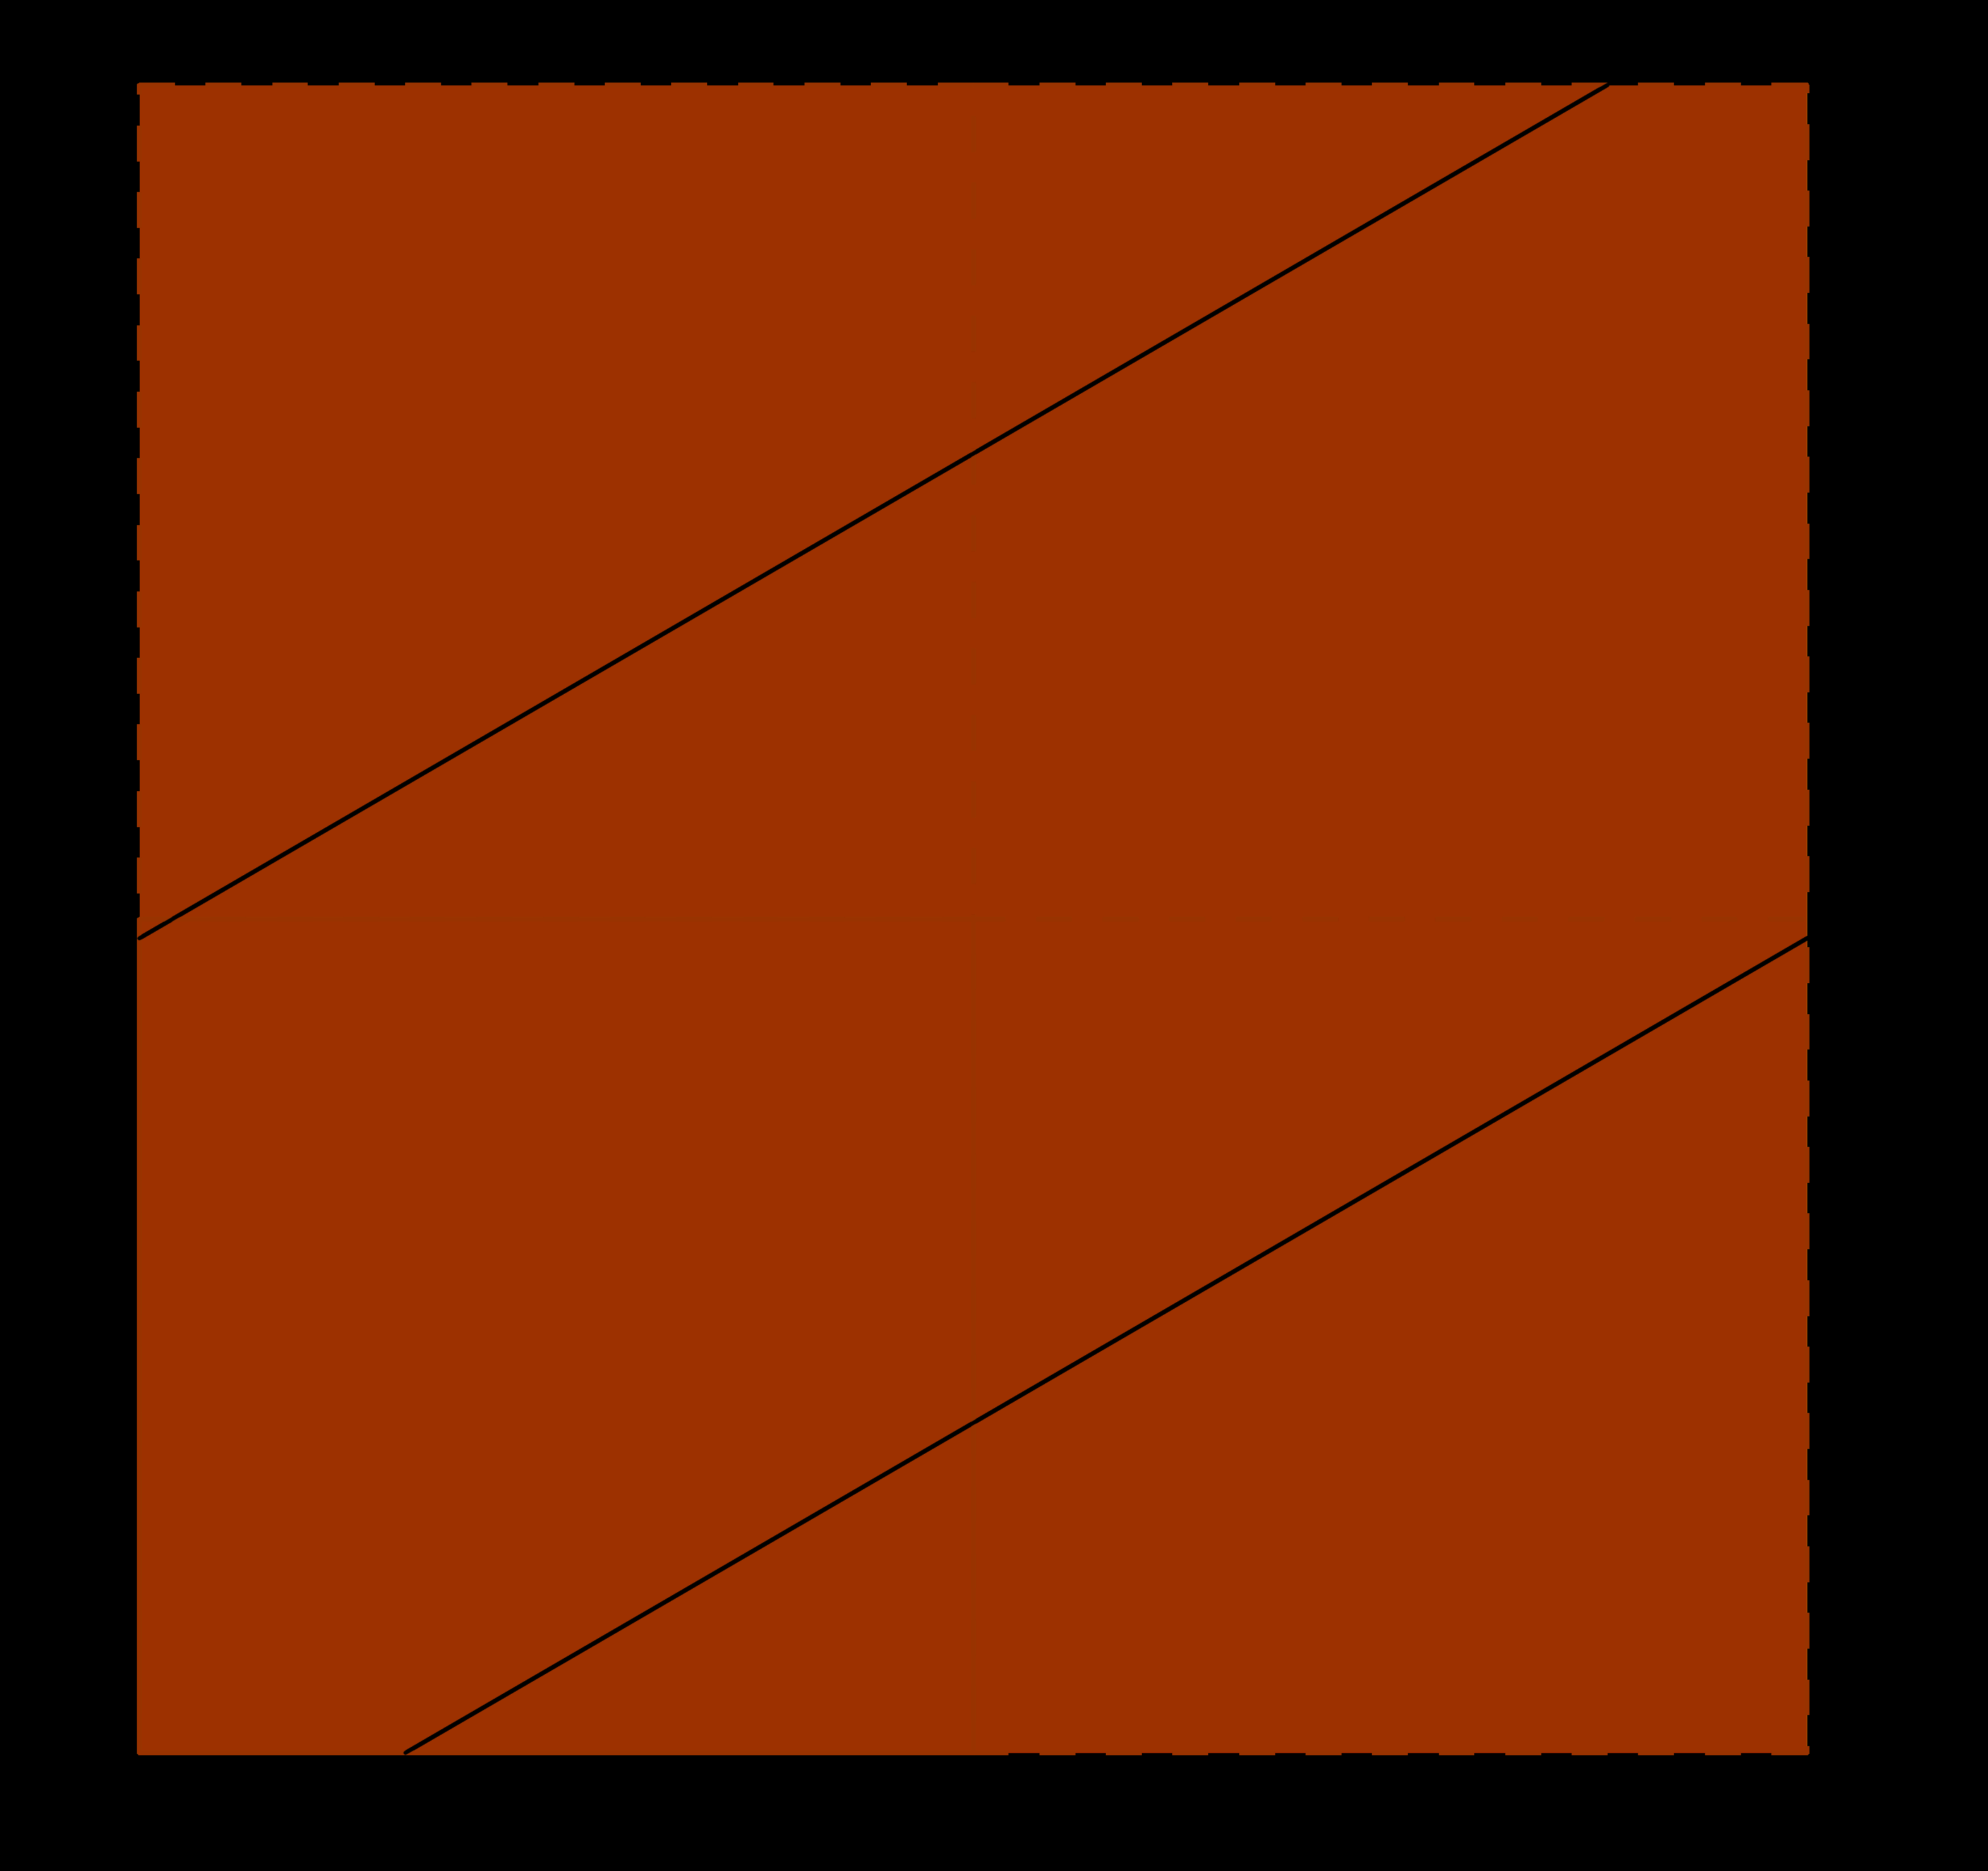
\includegraphics{flot-tore.png}
\caption{Dynamique sur le tore}
\end{figure}
\end{frame}

\begin{frame}{Billards: un contexte où les surfaces de translation
apparaissent naturellement}
\protect\hypertarget{billards-un-contexte-ouxf9-les-surfaces-de-translation-apparaissent-naturellement}{}
\begin{figure}
\centering
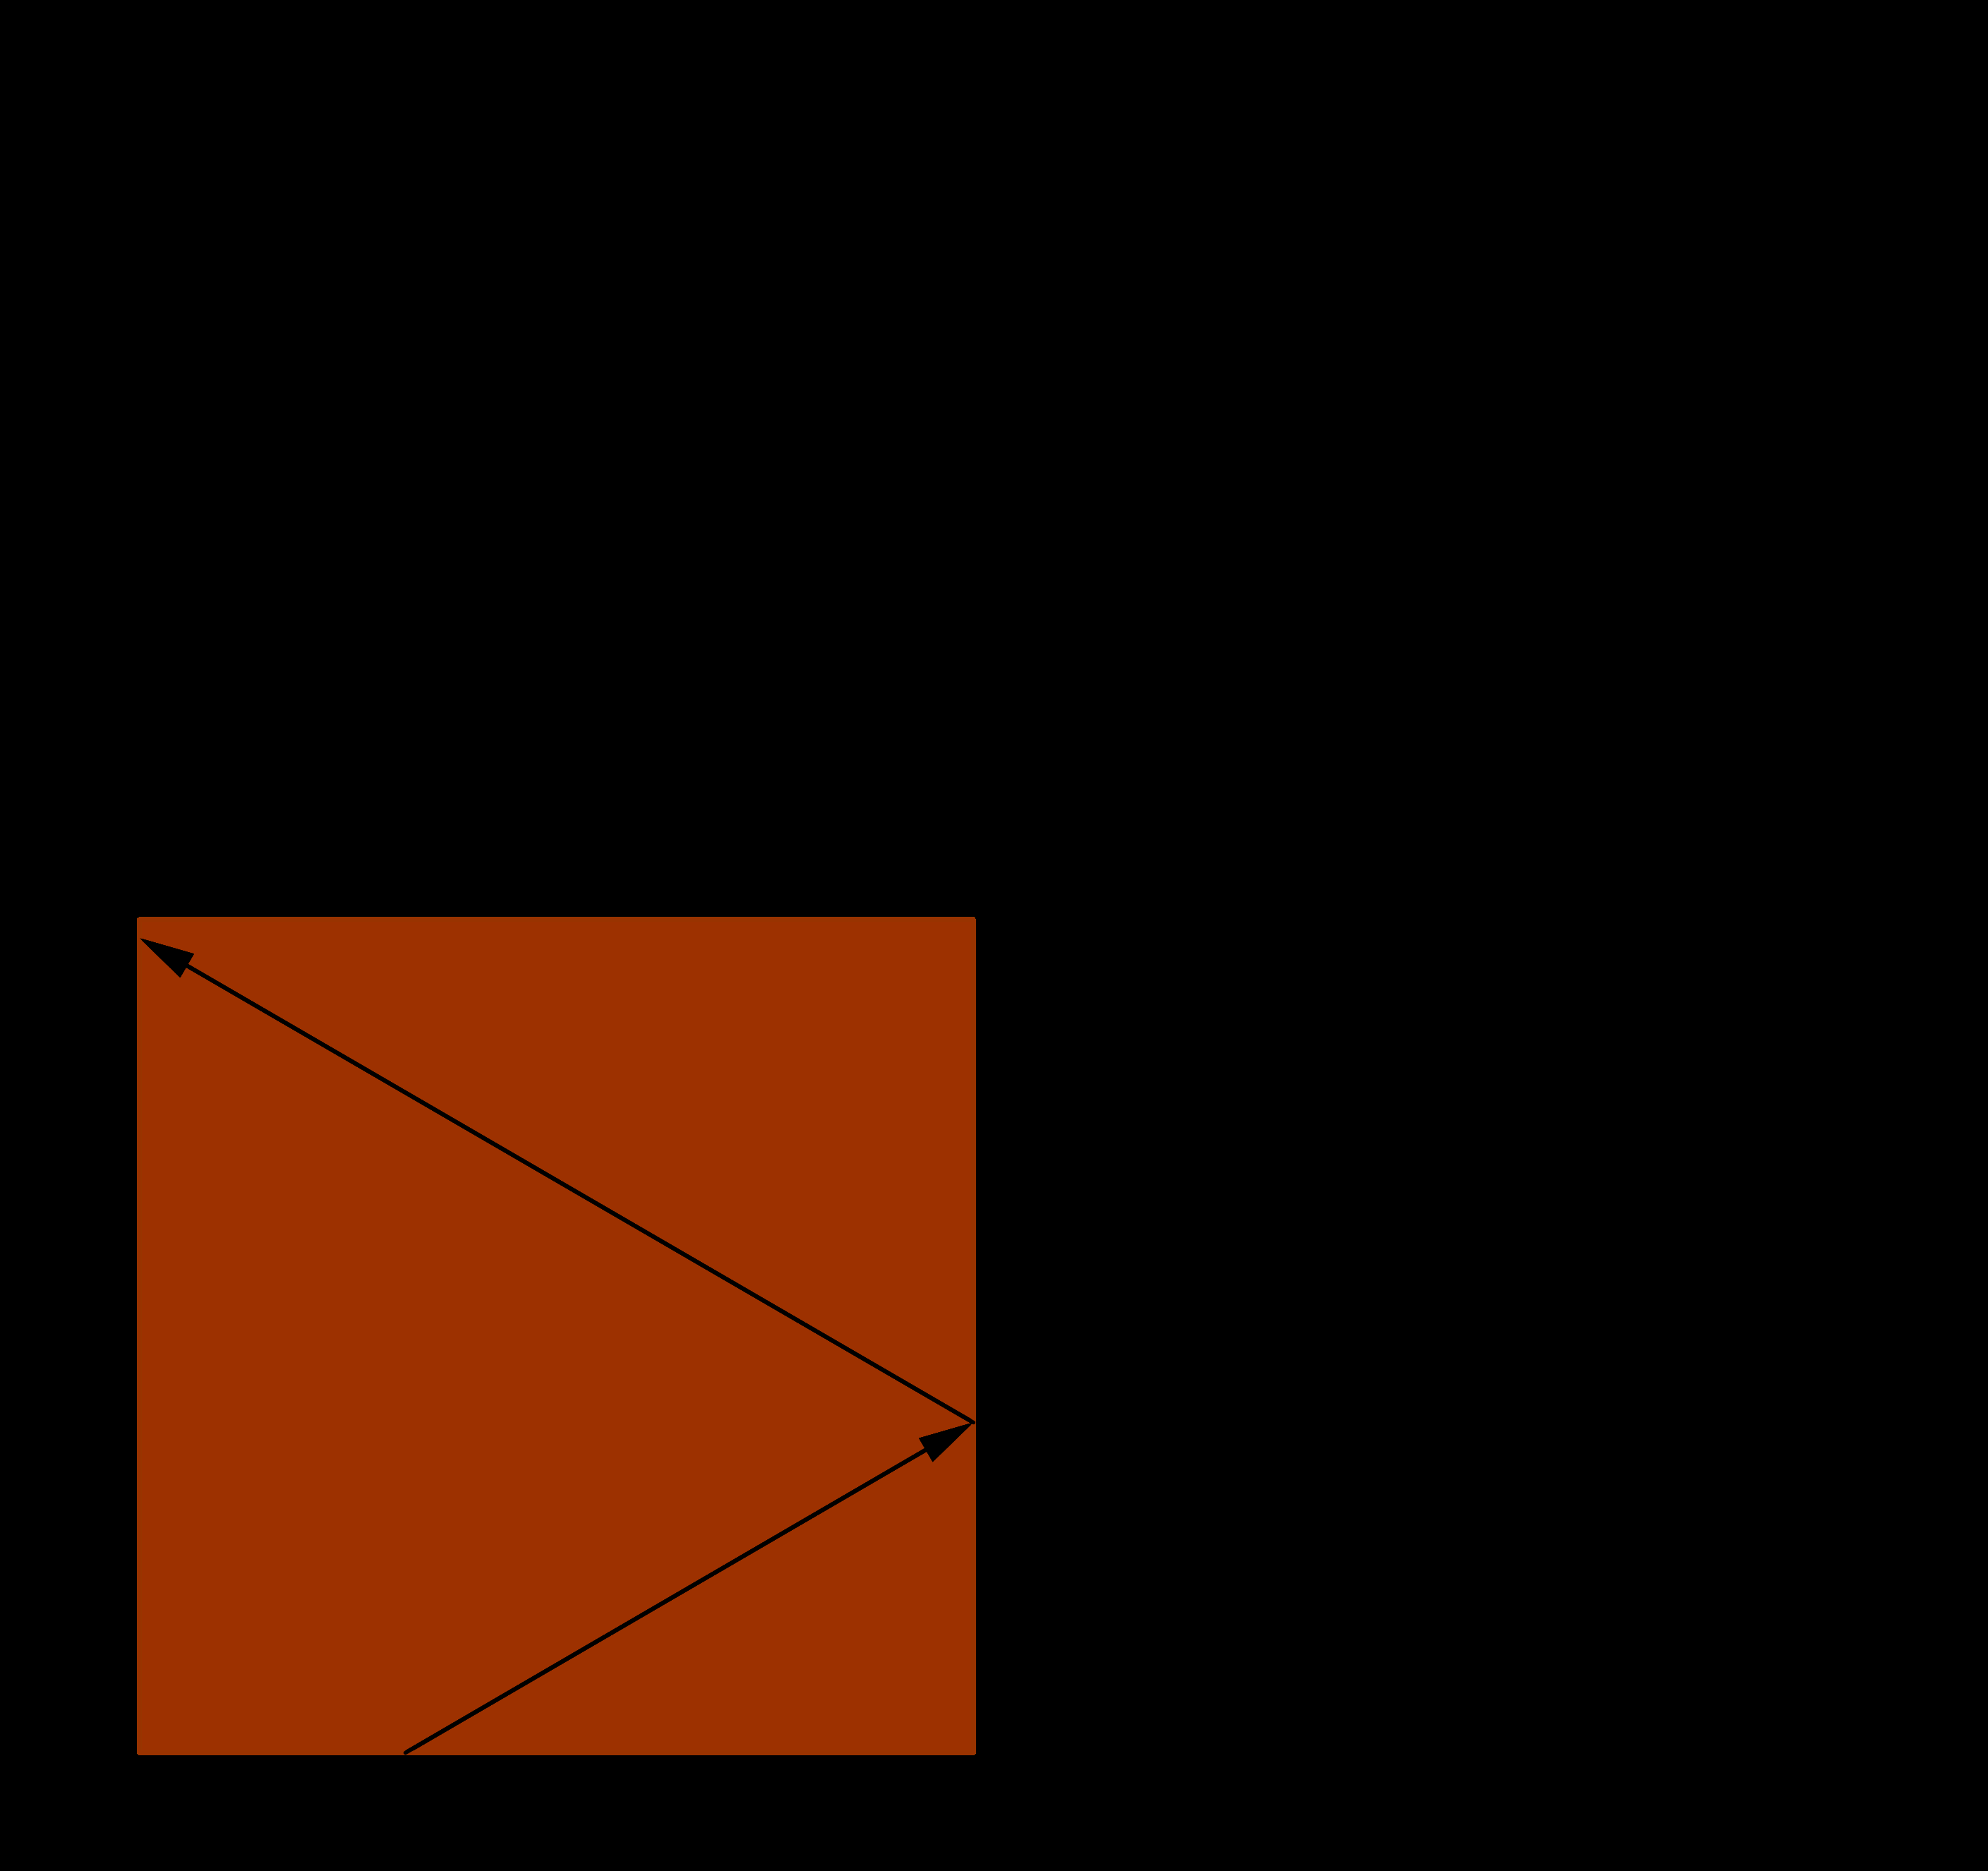
\includegraphics{rebond-carre.png}
\caption{rebond-carre.png}
\end{figure}
\end{frame}

\begin{frame}
\begin{figure}
\centering
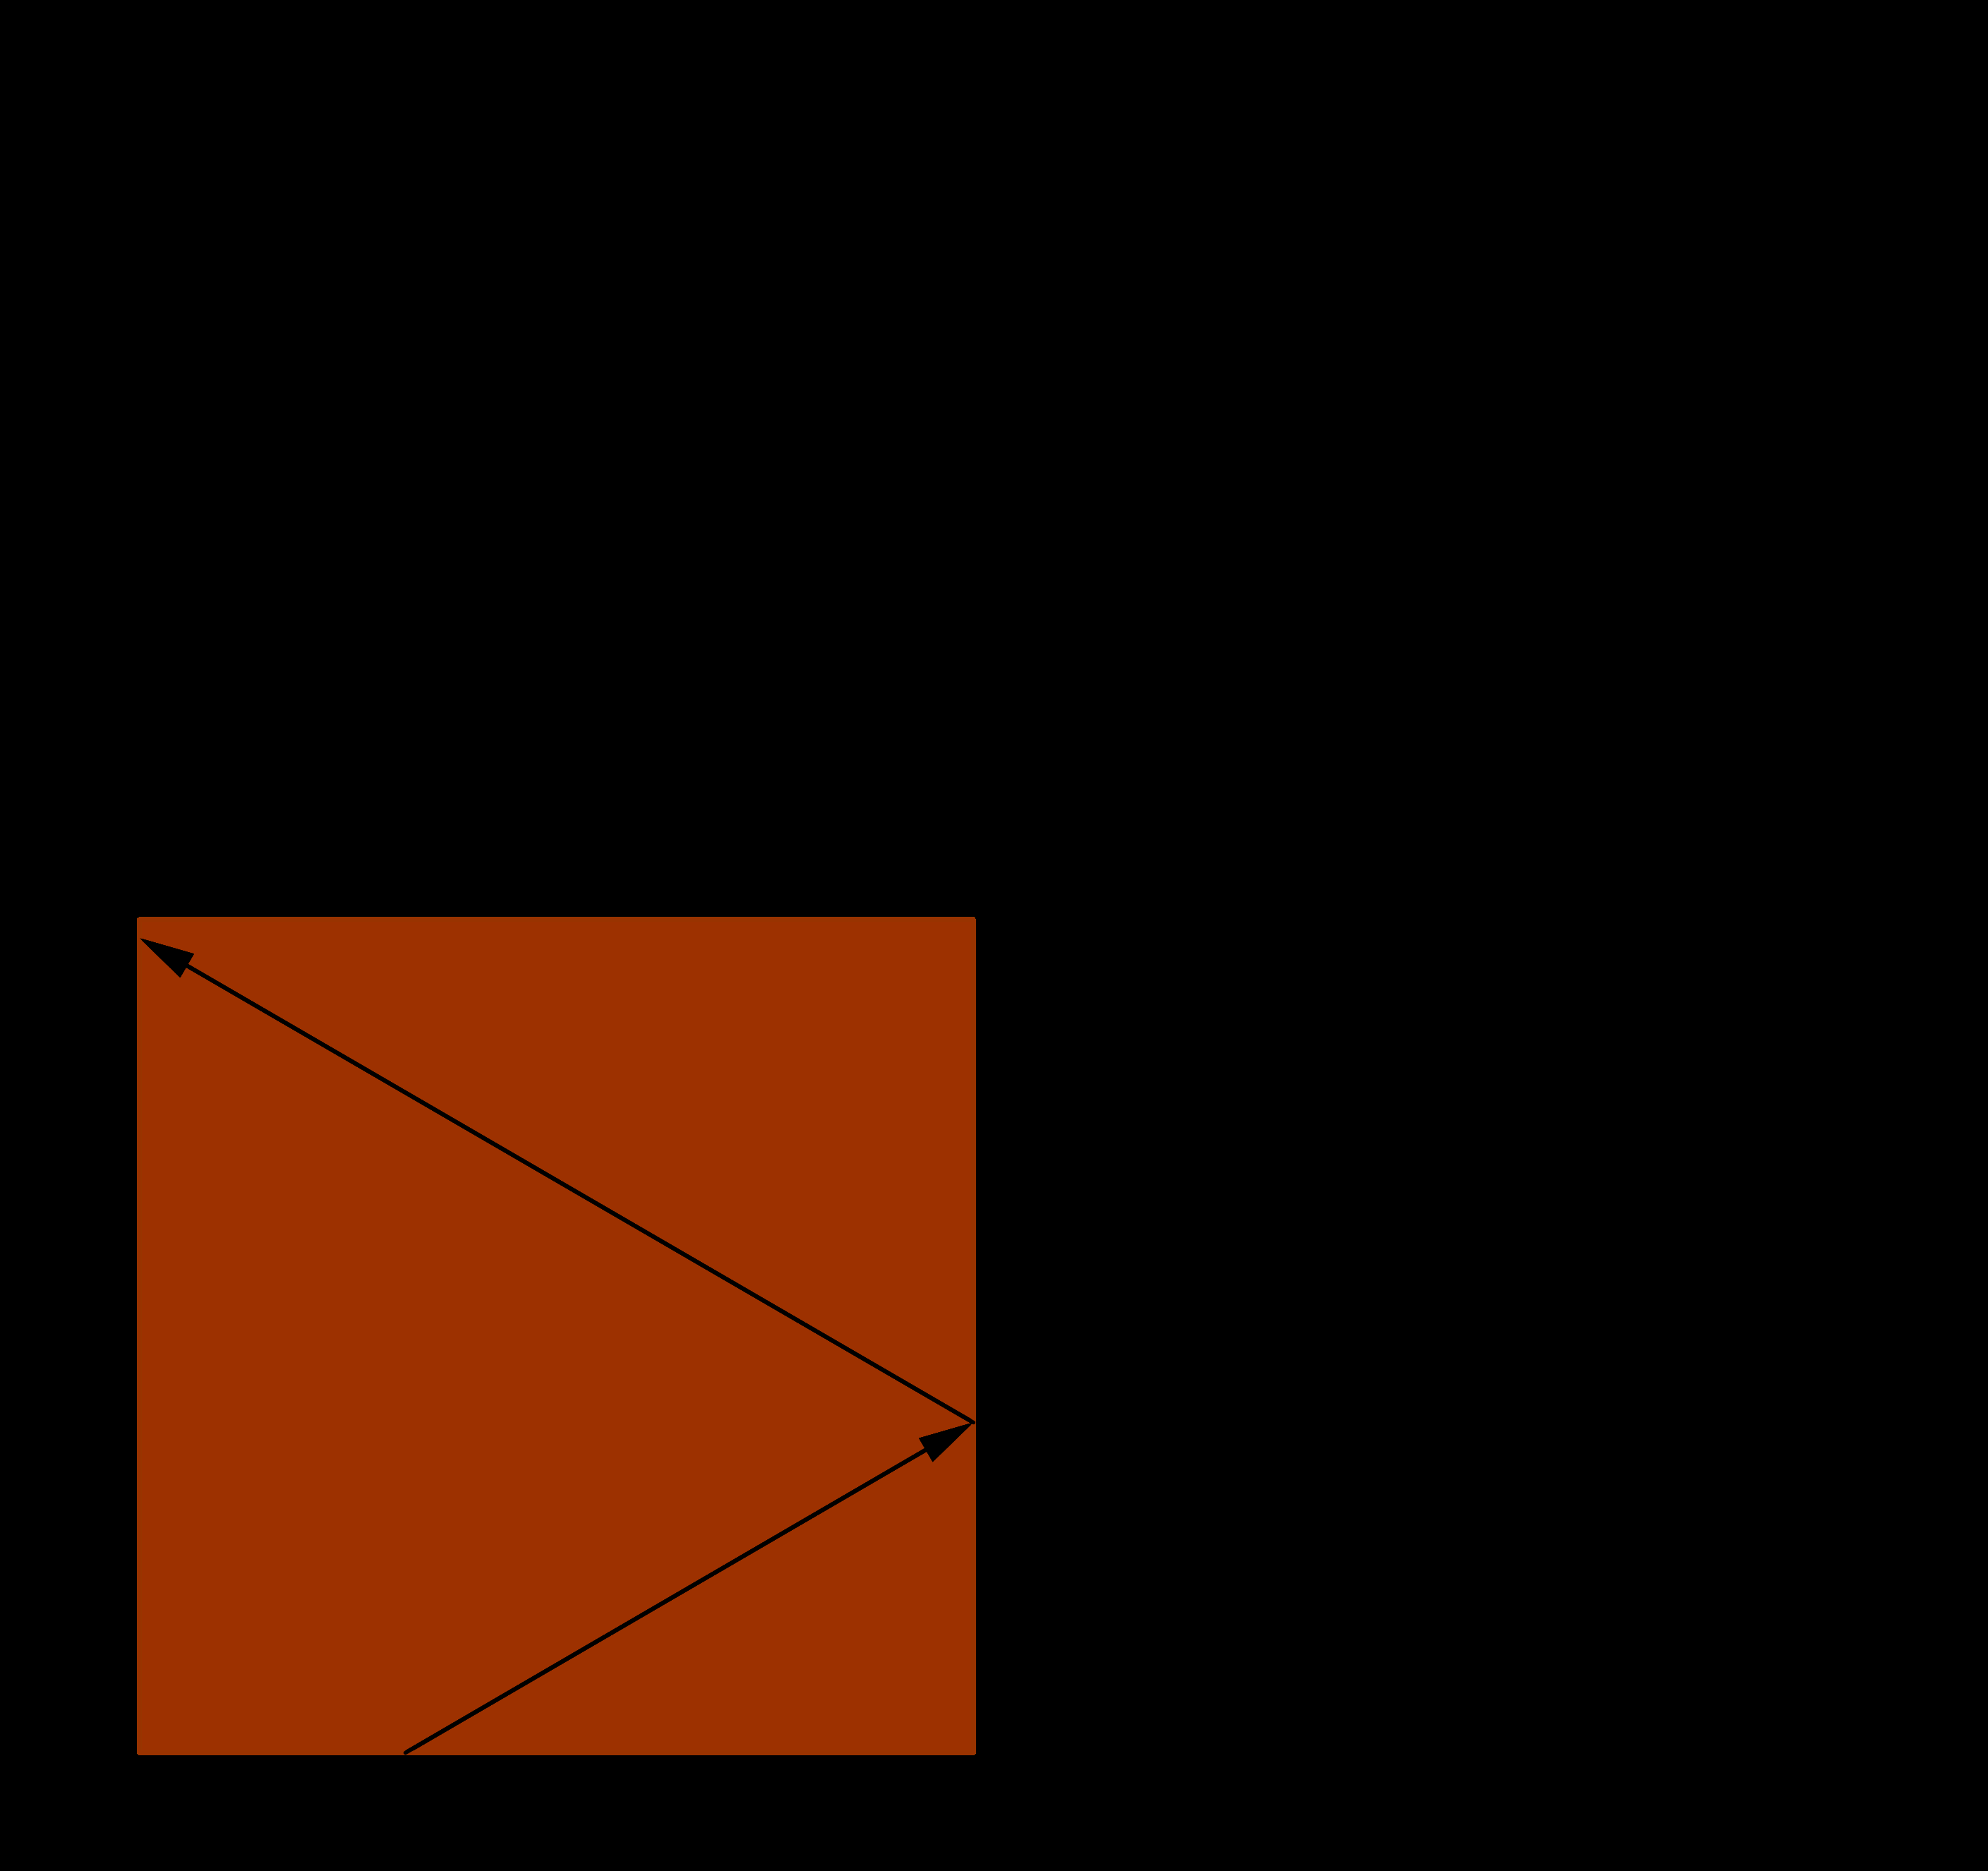
\includegraphics{rebond-carre.png}
\caption{rebond-carre.png}
\end{figure}
\end{frame}

\begin{frame}
\begin{figure}
\centering
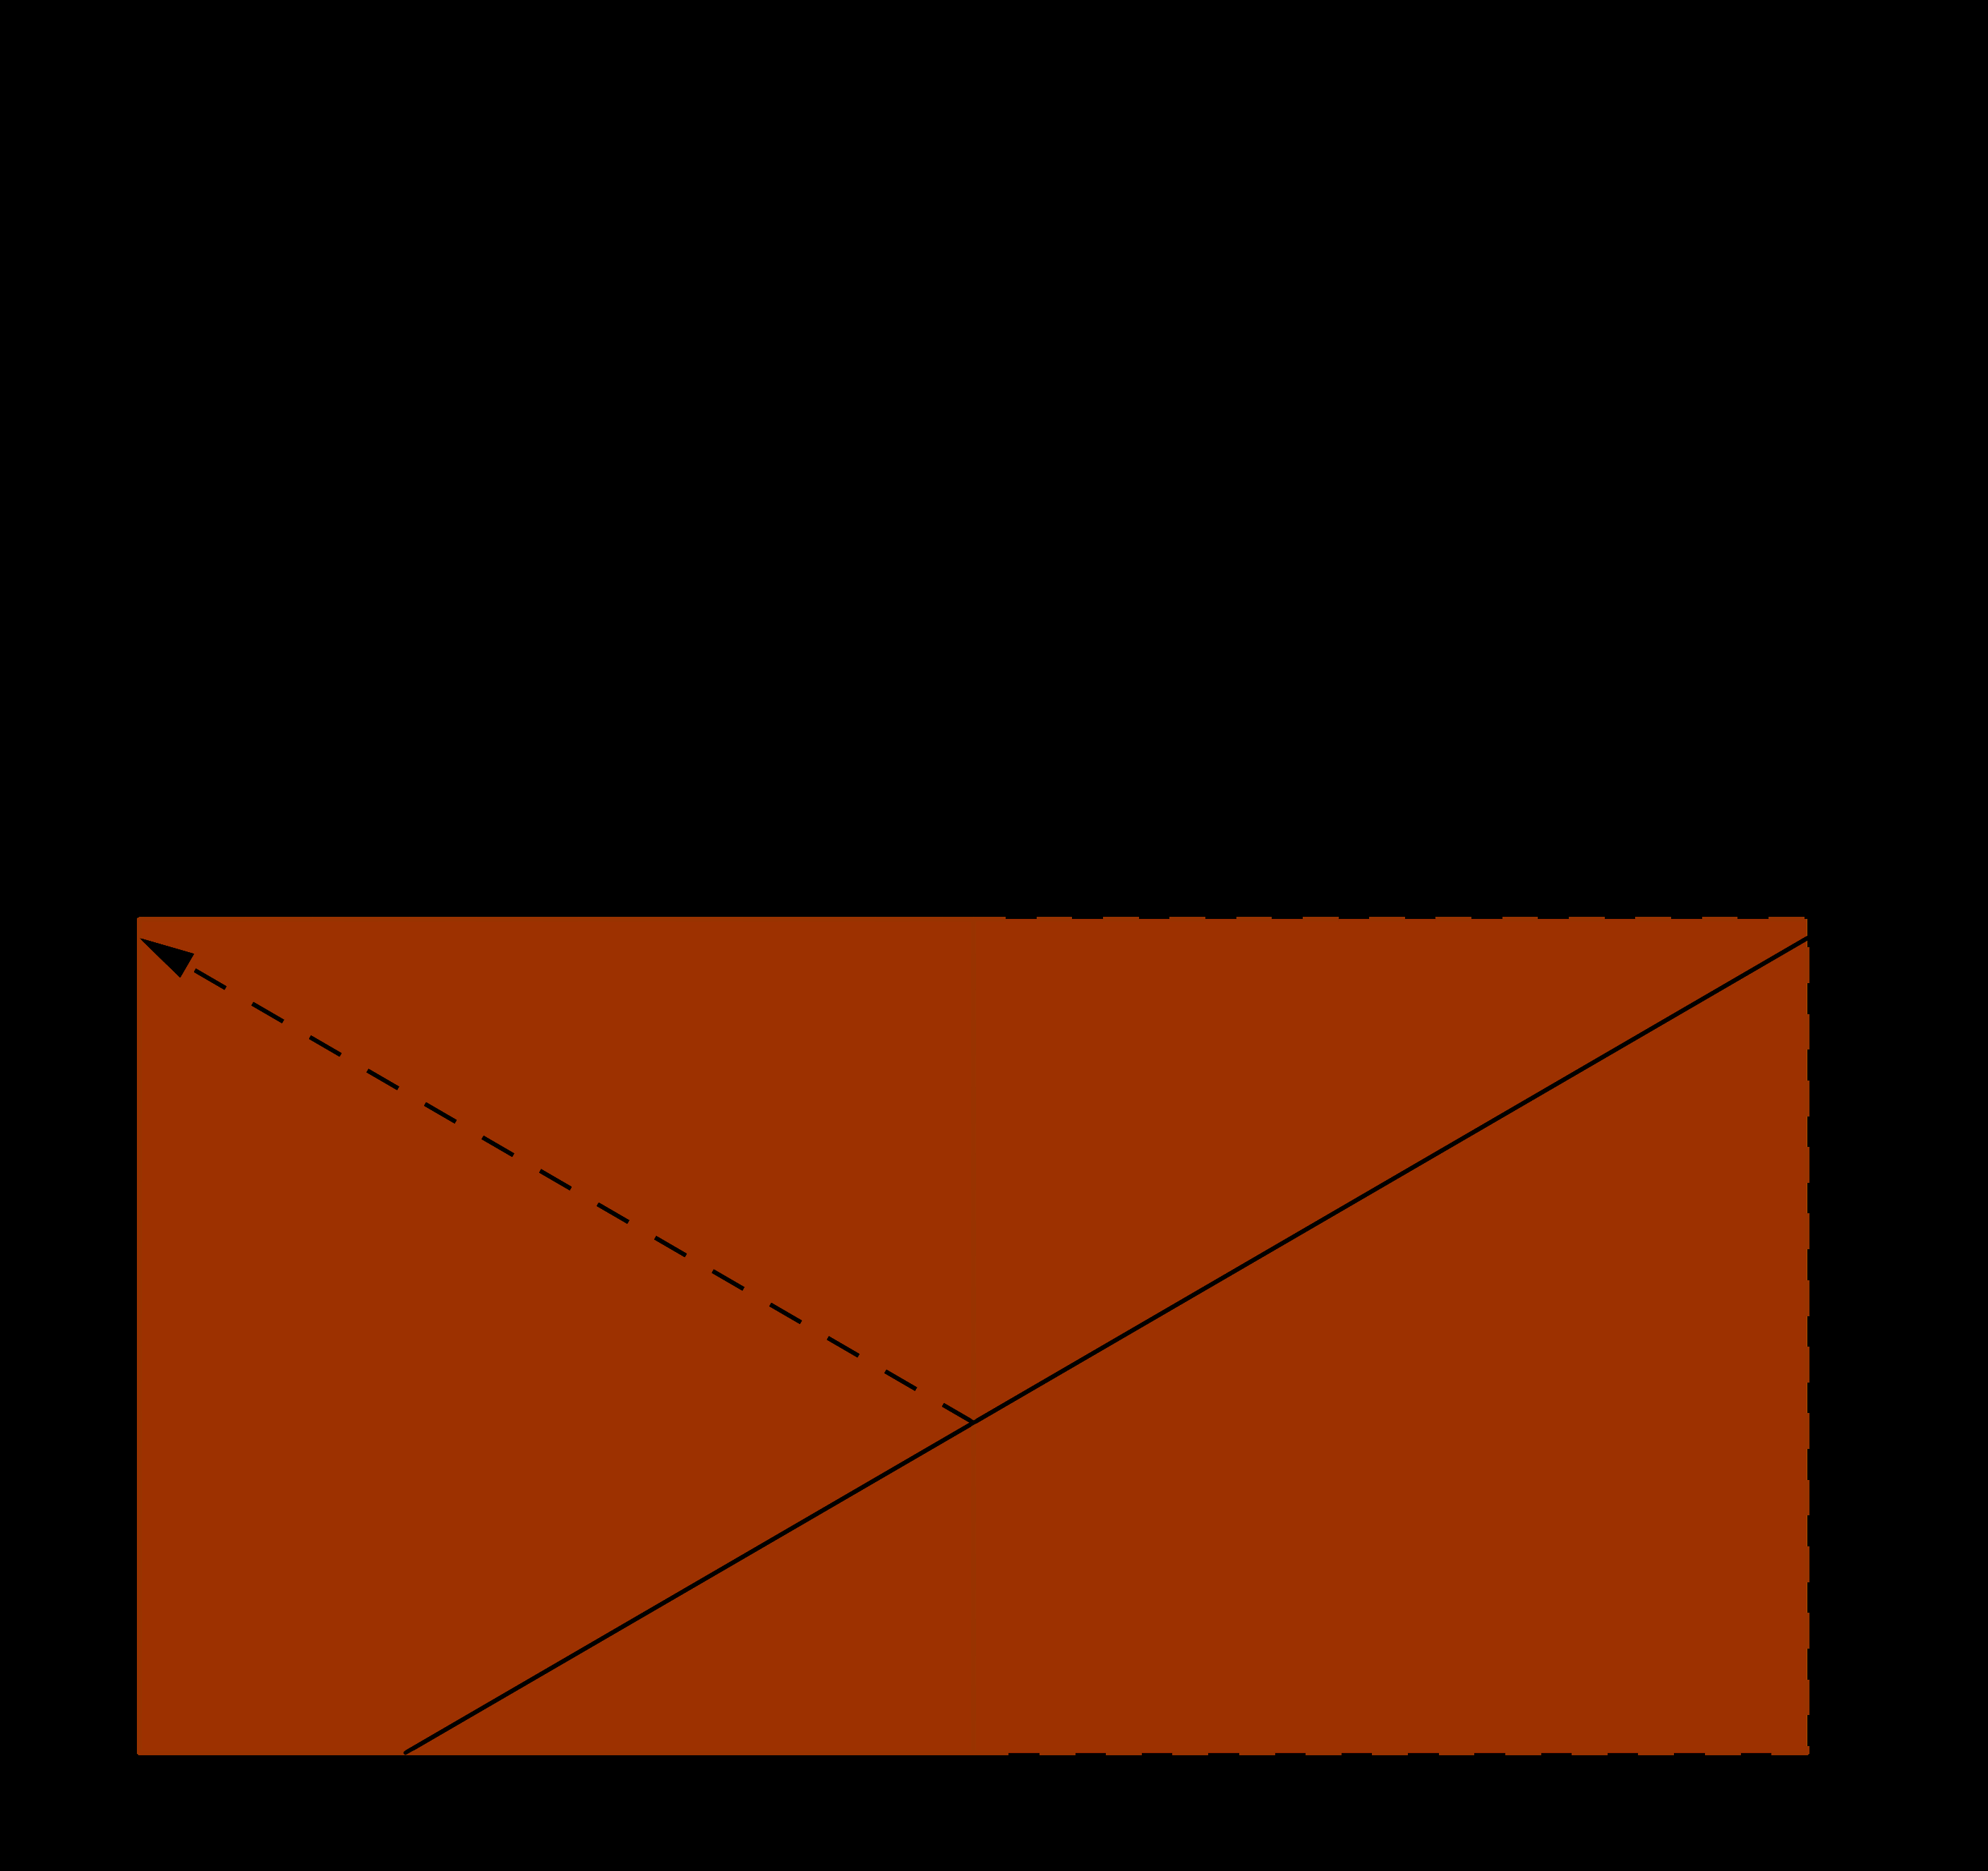
\includegraphics{depliage-2.png}
\caption{Commence à se deplier}
\end{figure}
\end{frame}

\begin{frame}
\begin{figure}
\centering
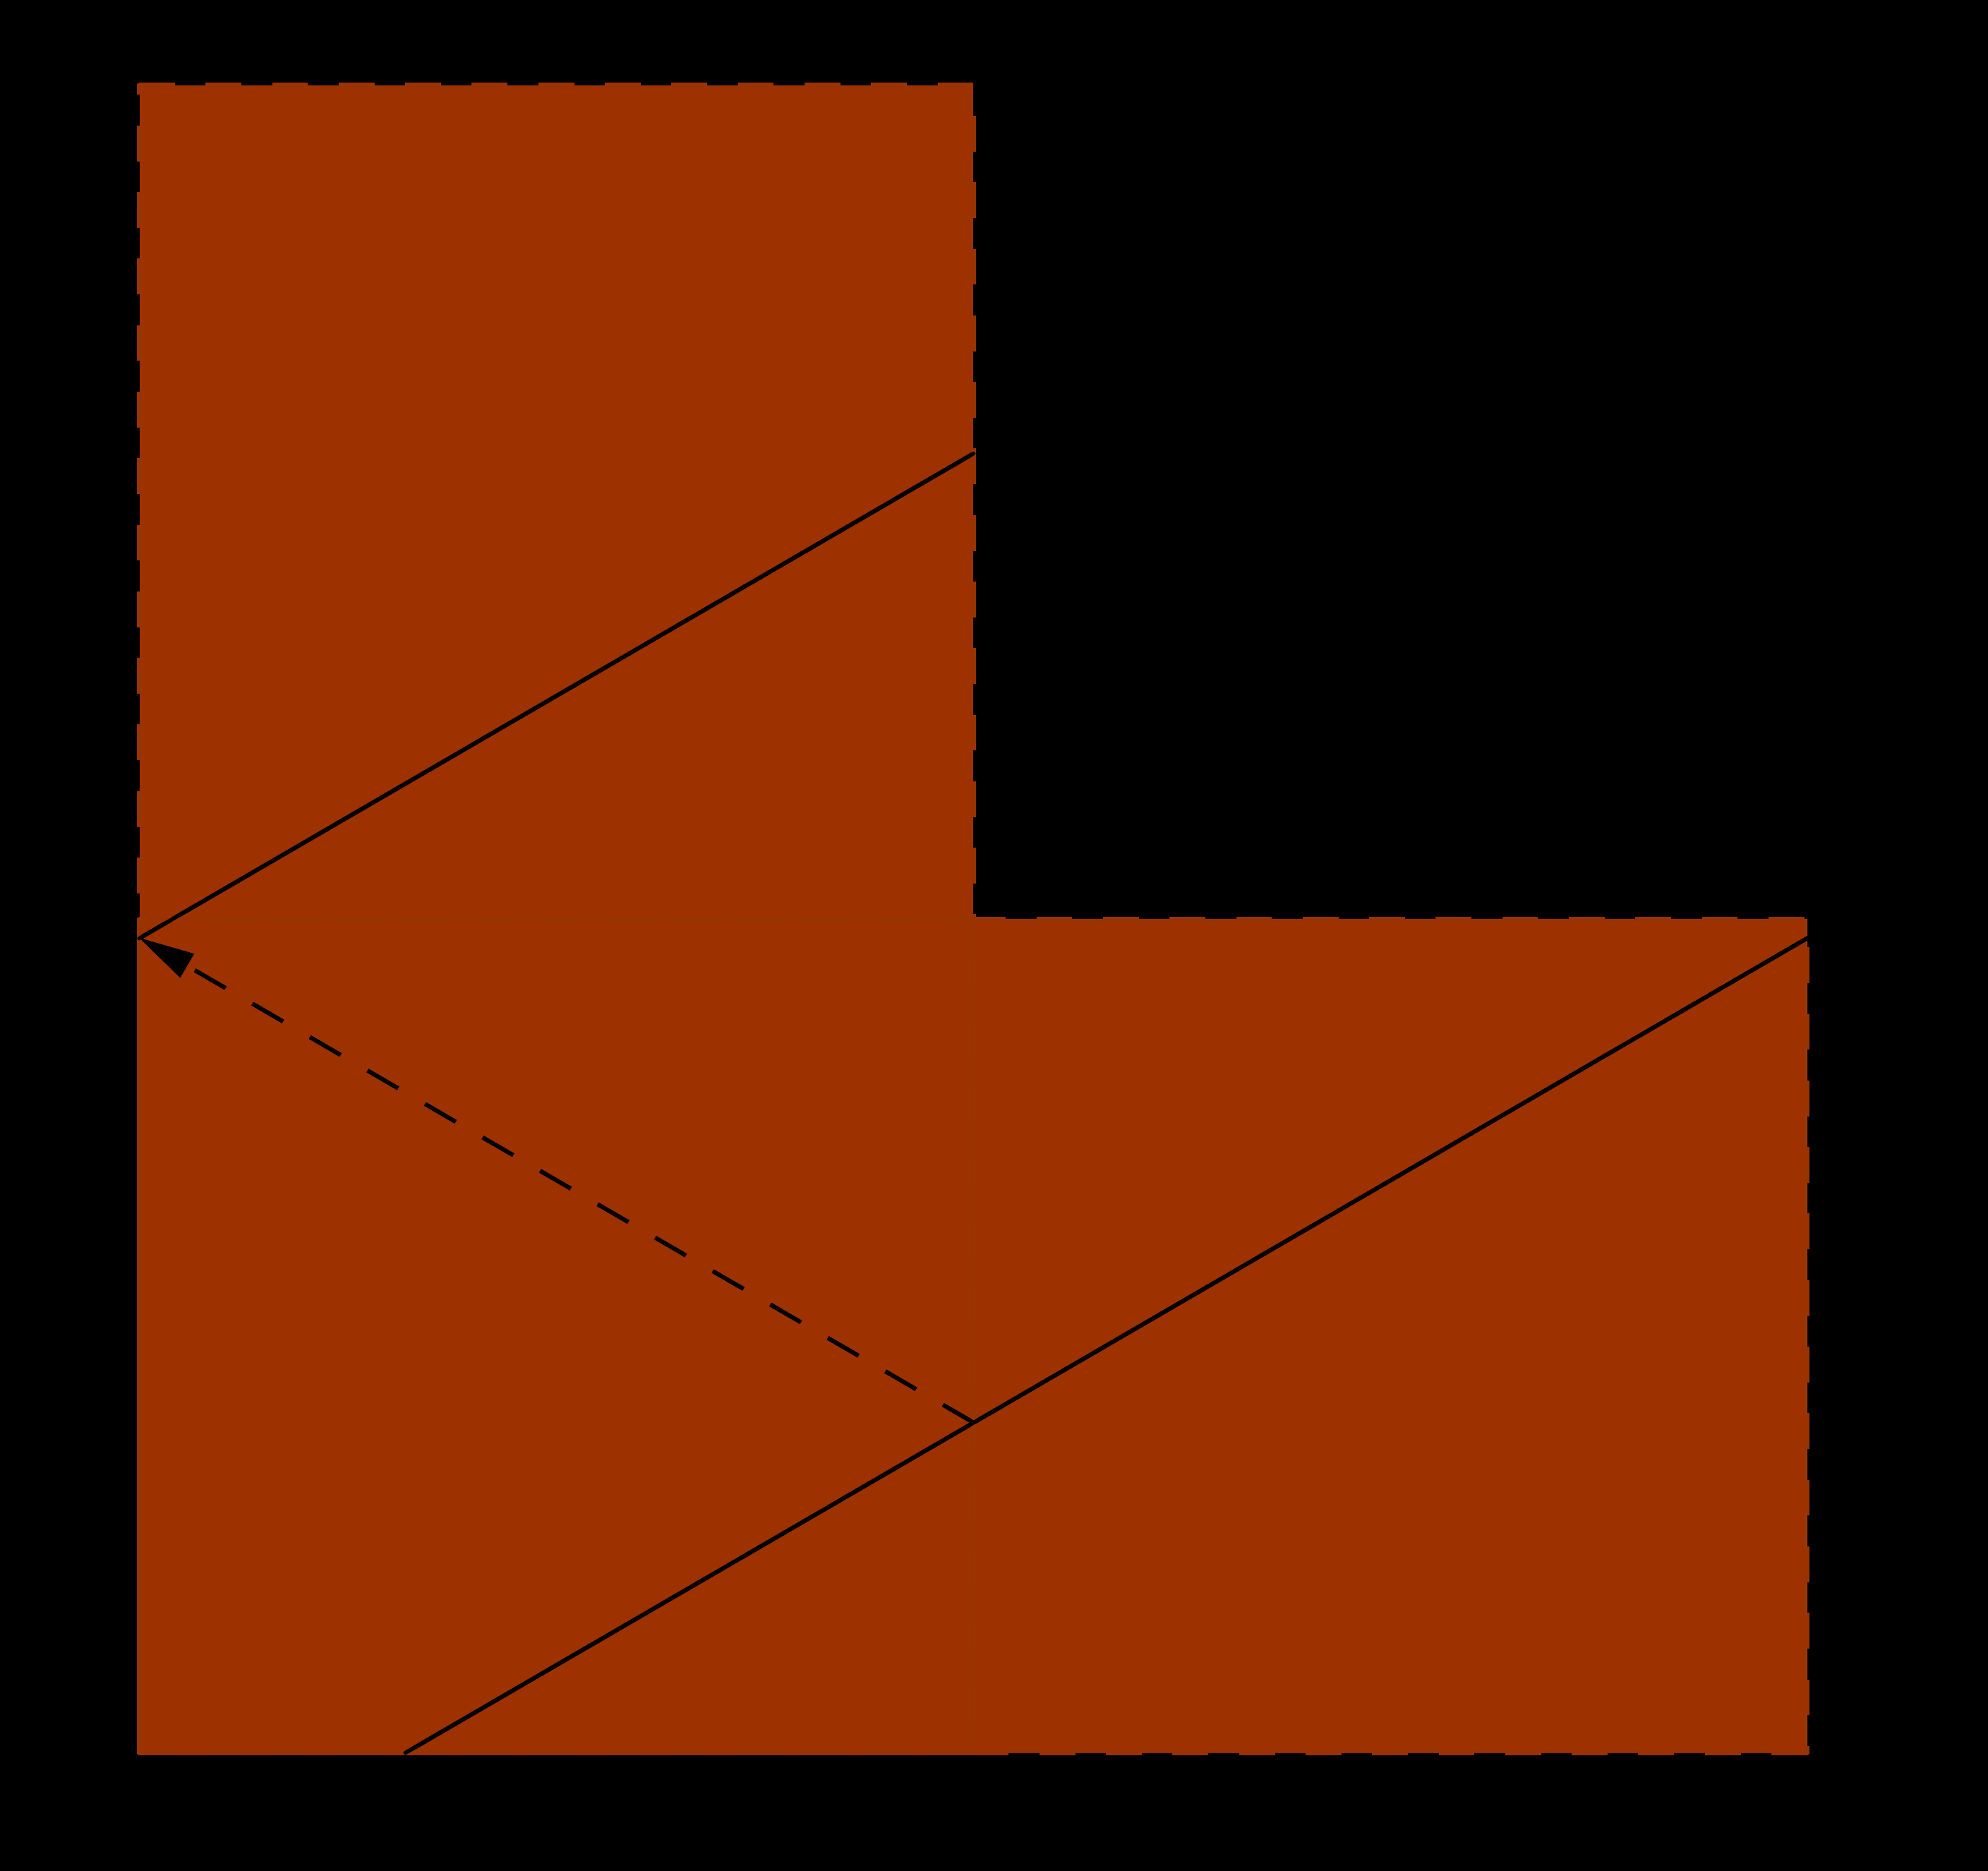
\includegraphics{flot-L.png}
\caption{Continue}
\end{figure}
\end{frame}

\begin{frame}
\begin{figure}
\centering
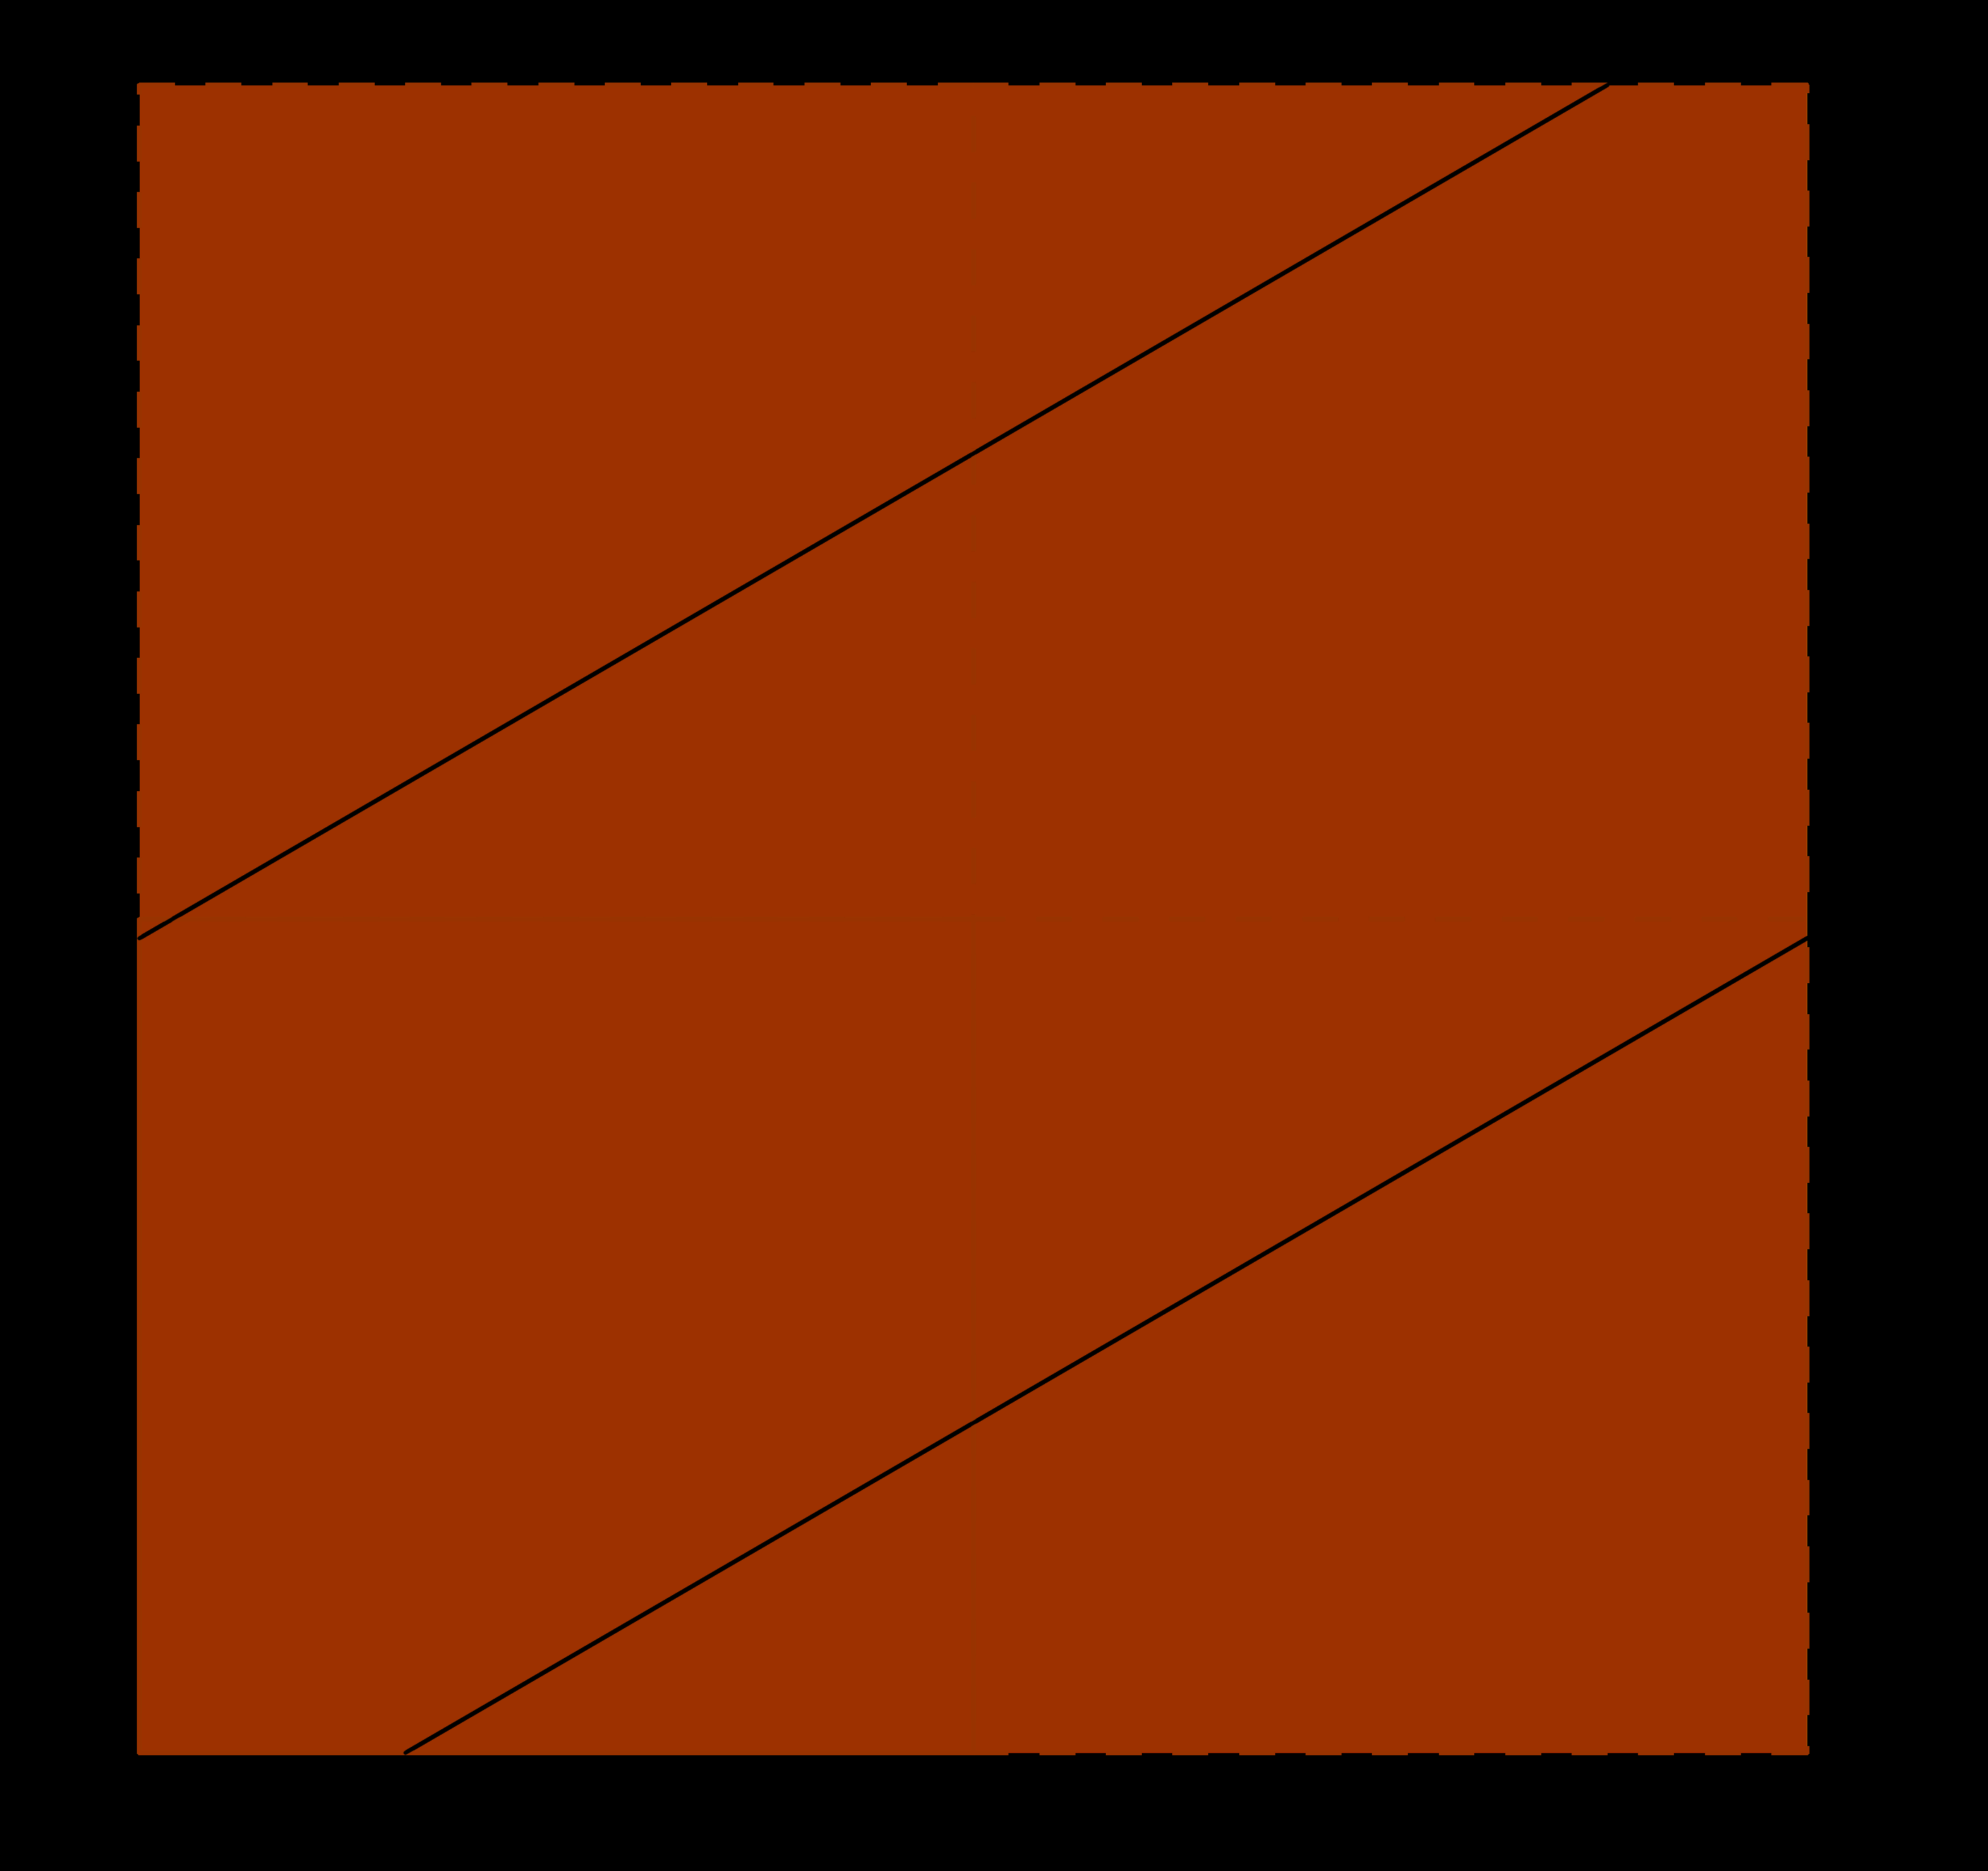
\includegraphics{flot-tore.png}
\caption{On obtient le flot sur le tore}
\end{figure}
\end{frame}

\begin{frame}{Questions ouvertes sur des billards polygonaux:}
\protect\hypertarget{questions-ouvertes-sur-des-billards-polygonaux}{}
\begin{itemize}
\tightlist
\item
  il existe toujours des trajectoires périodiques ?
\item
  toutes les trajectoires sont denses ? (\textbf{minimalité})
\item
  il y a ou pas des partitions non triviales (en mesure) en
  sous-ensembles invariants ? (\textbf{ergodicité})
\end{itemize}

\begin{figure}
\centering
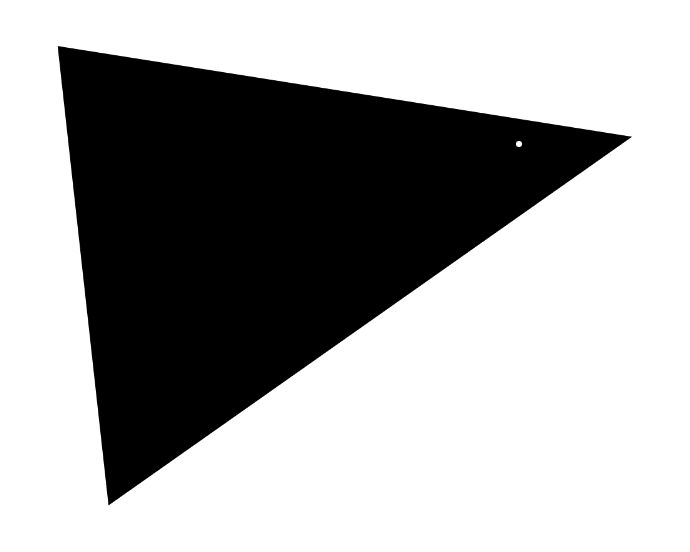
\includegraphics{triangle-1.png}
\caption{triangle-1.png}
\end{figure}

La troisième question de cette liste était le point de départ de ma
thèse, effectuée de 2011 à 2014 à Orsay sous la direction de
Jean-Christophe Yoccoz. La question est encore ouverte, he he, c'est à
dire que finalement dans ma thèse je réponds à d'autres questions
(moralement) en rapport avec celle-ci.
\end{frame}

\begin{frame}{Cylindres discrets - motivation}
\protect\hypertarget{cylindres-discrets---motivation}{}
\begin{figure}
\centering
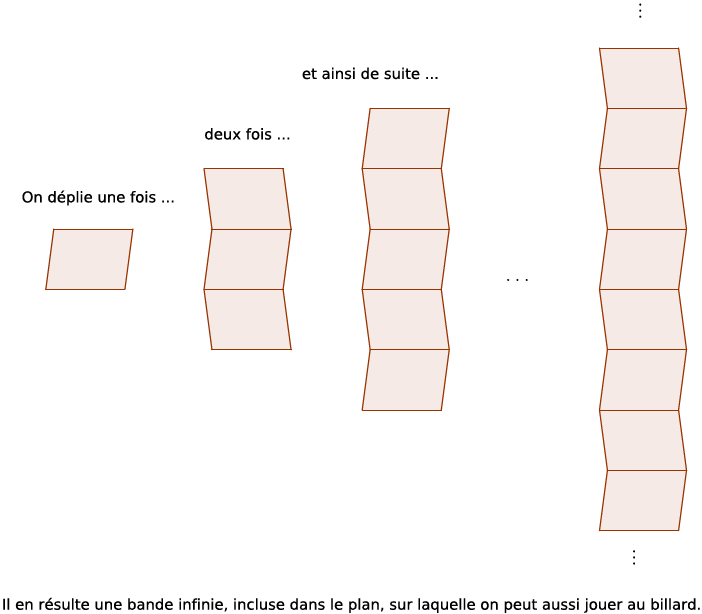
\includegraphics{parallelogramme-deplie-n-fois.png}
\caption{Parallélogramme deplié partiellement}
\end{figure}
\end{frame}

\begin{frame}
\begin{figure}
\centering
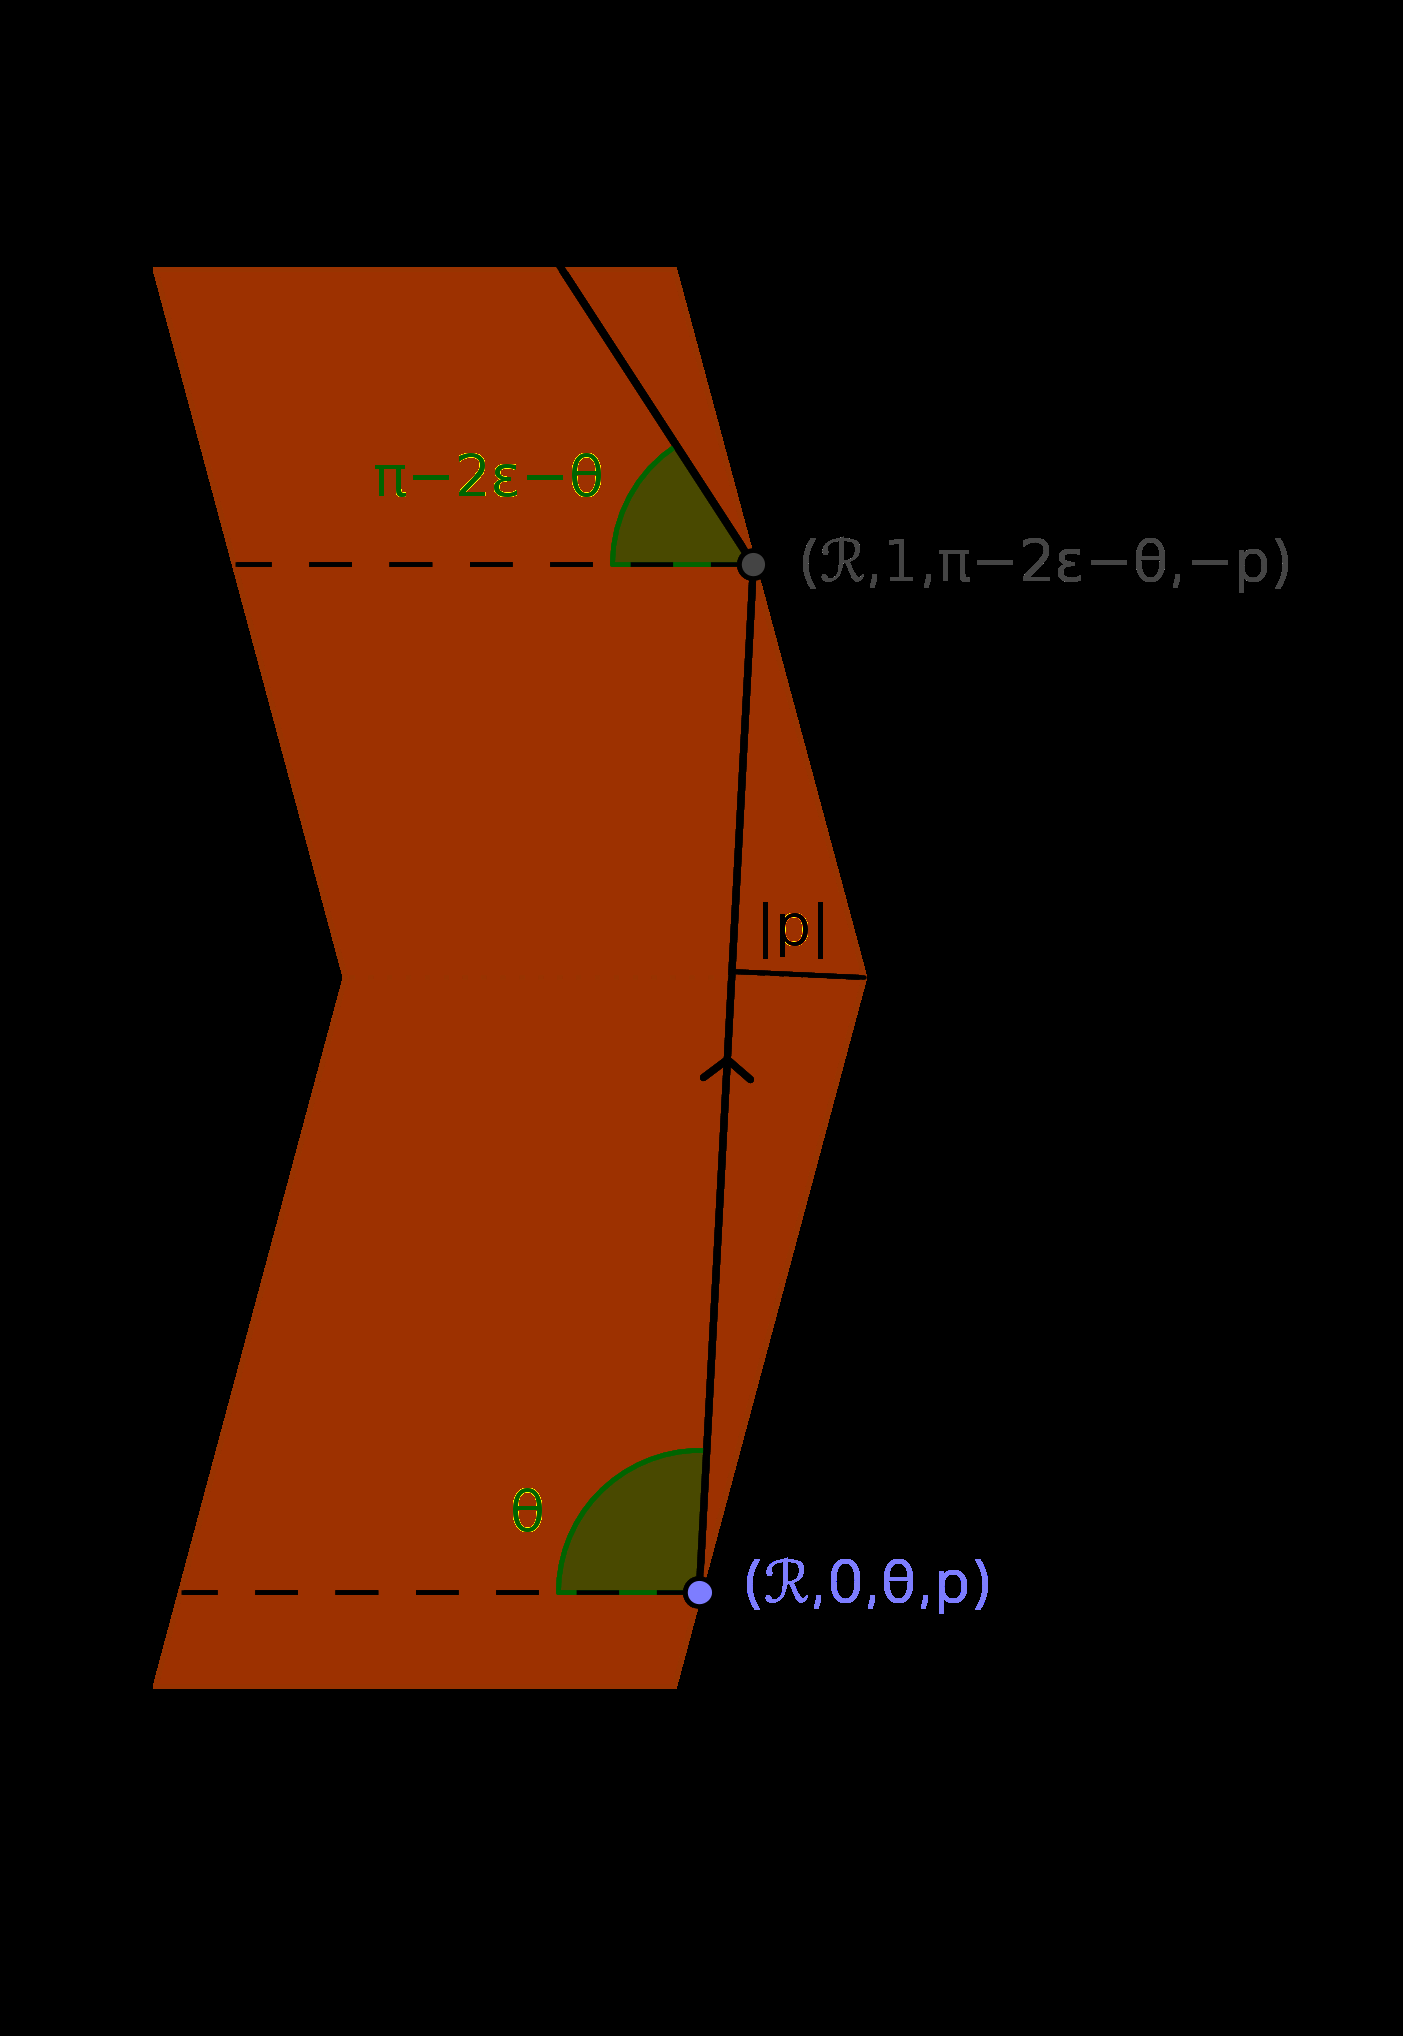
\includegraphics{rebond-cas-special.png}
\caption{rebond-cas-special.png}
\end{figure}

Similarité avec des familles d'applications sur le cylindre discret
\(ℤ×𝕋\). L'étude de la dynamique de ces applications fût finalement
l'objet de ma thèse.
\end{frame}

\begin{frame}{Une famille de transformations du cylindre discret
\(ℤ×𝕋\)}
\protect\hypertarget{une-famille-de-transformations-du-cylindre-discret-ux2124ux1d54b}{}
Considérons une suite bi-infinie de paramètres de rotation
\(α_n∈𝕋 = [0,1]/\{0\sim 1\}\). Pour chaque suite de la sorte, appliquons
la rotation par \(α_n\) au cercle \(\{n\}×𝕋\). Puis, coupons tous les
cercles en deux intervalles de même longueur, independants des
paramètres de rotation, et considérons leur intérieur, qu'on appelera la
partie descendante, et la partie montante, puis déplaçons la partie de
droite de un niveau vers le haut et la partie de gauche d'un niveau vers
le bàs.

Ainsi, à chaque suite bi-infinie \((α_n)_{n∈ℤ}\) correspond une
transformation du cylindre discret \(ℤ×𝕋\), définie partout sauf sur un
ensemble discret de points singuliers ( ceux qui après rotation
arriveraient sur les bords des parties montantes et descendants). C'est
cette famille de transformations \(T_{α_n}\) que j'ai étudié dans ma
thèse.
\end{frame}

\begin{frame}{Dynamique générique d'une famille de transformations de
\(ℤ×𝕋\)}
\protect\hypertarget{dynamique-guxe9nuxe9rique-dune-famille-de-transformations-de-ux2124ux1d54b}{}
Espace de paramètres \(𝕋^n\), dispose d'une mesure de probabilité et
d'une topologie produit.

Pour simplifier les notations, on va écrire \(α\) pour la suite
\((α_n)_{n\in ℤ}\). Dans ma thèse j'ai demontré que:

\begin{itemize}
\item
  presque sùrement, \(T_α\) n'a pas d'ensemble errant de mesure positive
\item
  génériquement:

  \begin{itemize}
  \tightlist
  \item
    \(T_α\) est conservative
  \item
    toute demi-orbite \(T_α\) définie pour une infinité d'itérations est
    dense (c-à-d \(T_α\) est \textbf{minimal})
  \item
    tout sous-ensemble invariant par \(T_α\) est de mesure nulle ou bien
    a un complement de mesure nulle (c-à-d \(T_α\) est
    \textbf{ergodique})
  \end{itemize}
\end{itemize}
\end{frame}

\begin{frame}{Techniques developpées dans la thèse}
\protect\hypertarget{techniques-developpuxe9es-dans-la-thuxe8se}{}
Pour montrer ces résultats, je me suis appuyé sur des résultats bien
connus pour des échanges d'intervalles, pour lesquelles les propriétés
dynamiques que j'étudiais était déjà bien connues:

\textbf{Thm (Poincaré)} Tout système dynamique de mesure finie est
conservatif.

\textbf{Thm (Keane)} Tout échange d'intervalles ``irréductible'' est
minimal.

\textbf{Thm (Masur-Tabachnikov)} Tout échange d'intervalle minimal est
aussi ergodique.

Ensuite, j'ai procédé par perturbations: des valeurs spéciales de
\(α_n=±½\), (c-à-d les rotations par un demi-tour), permettent d'obtenir
des sous-ensembles dans l'espace des phases qui sont invariants et qui
sont des échanges d'intervalles classiques. Ensuite, en traduit la
propriété dynamique qu'on veut montrer dans une formule quantitative et
puis on construit des ouverts denses autour de ces paramètres spéciaux
en prenant garde à ne pertuber qu'un petit peu cette formule.
\end{frame}

\begin{frame}{Les surfaces en escalier.}
\protect\hypertarget{les-surfaces-en-escalier.}{}
\begin{figure}
\centering
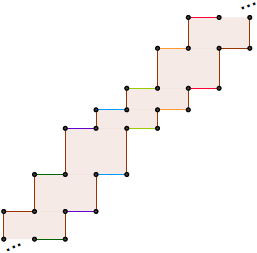
\includegraphics{escalier-hauteur-variable.png}
\caption{Escalier à hauteur variable}
\end{figure}
\end{frame}

\begin{frame}{Le modèle wind-tree des Ehrenfest:}
\protect\hypertarget{le-moduxe8le-wind-tree-des-ehrenfest}{}
\href{https://rantonse.no/demos/MirrorRoom/}{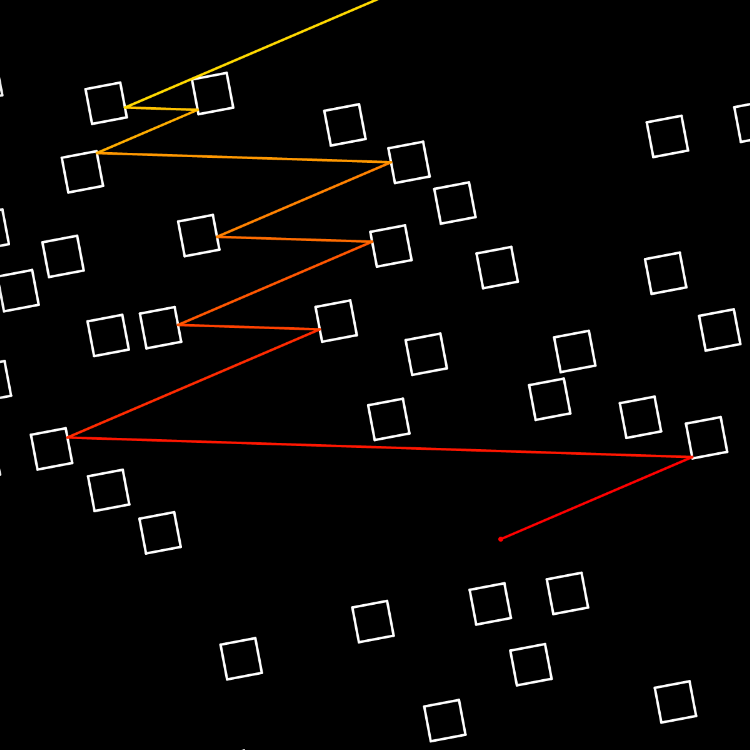
\includegraphics{wind-tree.png}}

Avec Serge Troubetzkoy, on a montré que génériquement, la dynamique du
wind-tree est minimale (2015), ergodique (2016), de puissances
cartésiennes ergodiques (2016-2017) et uniquement ergodique (2017-2019)
dans presque toute direction.
\end{frame}

\begin{frame}{Retour aux surfaces en escalier:}
\protect\hypertarget{retour-aux-surfaces-en-escalier}{}
\begin{figure}
\centering
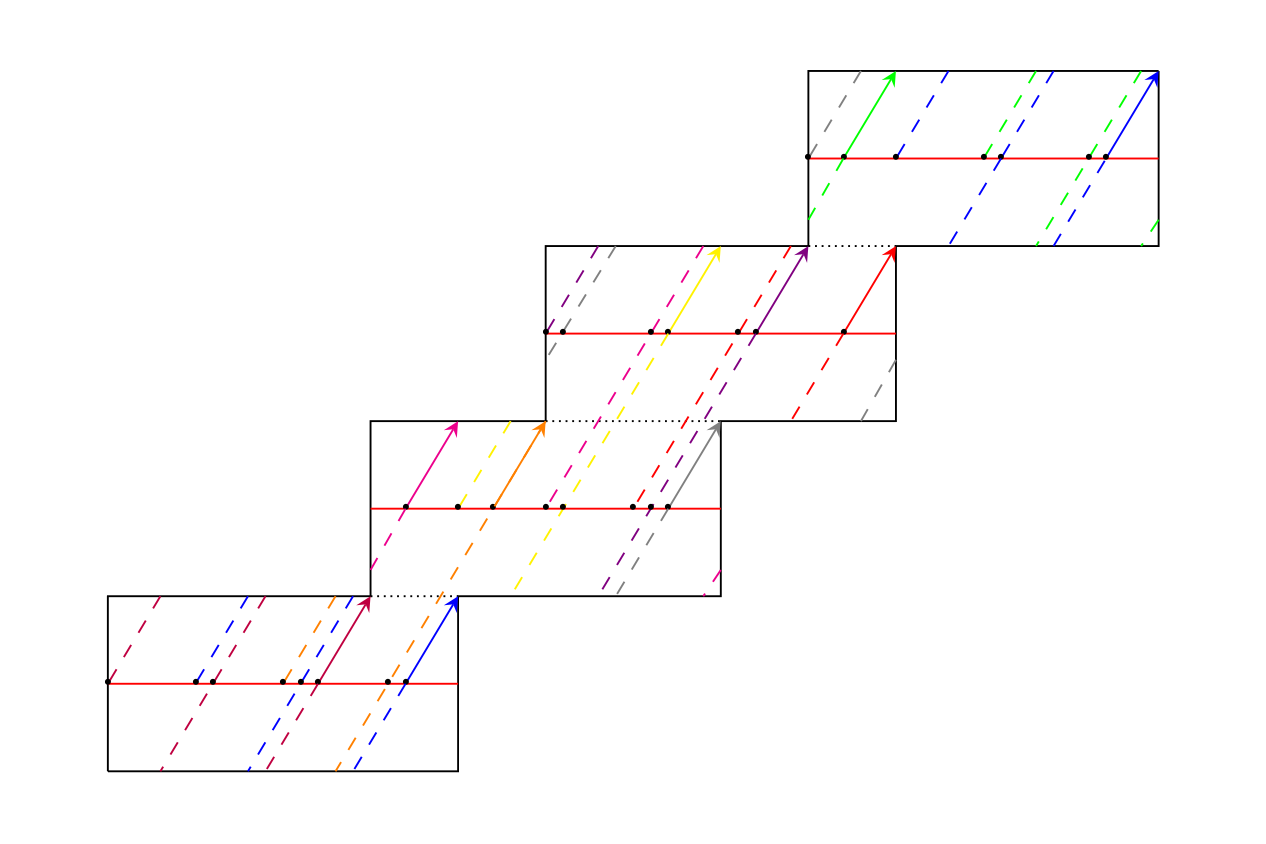
\includegraphics{orbites-escalier.png}
\caption{Orbites sur une surface en escalier à recouvrement variable}
\end{figure}
\end{frame}

\hypertarget{illustrations-des-mathuxe9matiques-et-intuxe9gration-dans-gamble}{%
\section{Illustrations des mathématiques et intégration dans
Gamble}\label{illustrations-des-mathuxe9matiques-et-intuxe9gration-dans-gamble}}

\begin{frame}{Tores plats et autres surfaces de translation pliées en
origami}
\protect\hypertarget{tores-plats-et-autres-surfaces-de-translation-pliuxe9es-en-origami}{}
\href{https://p3d.in/u/albamath/zJFfh}{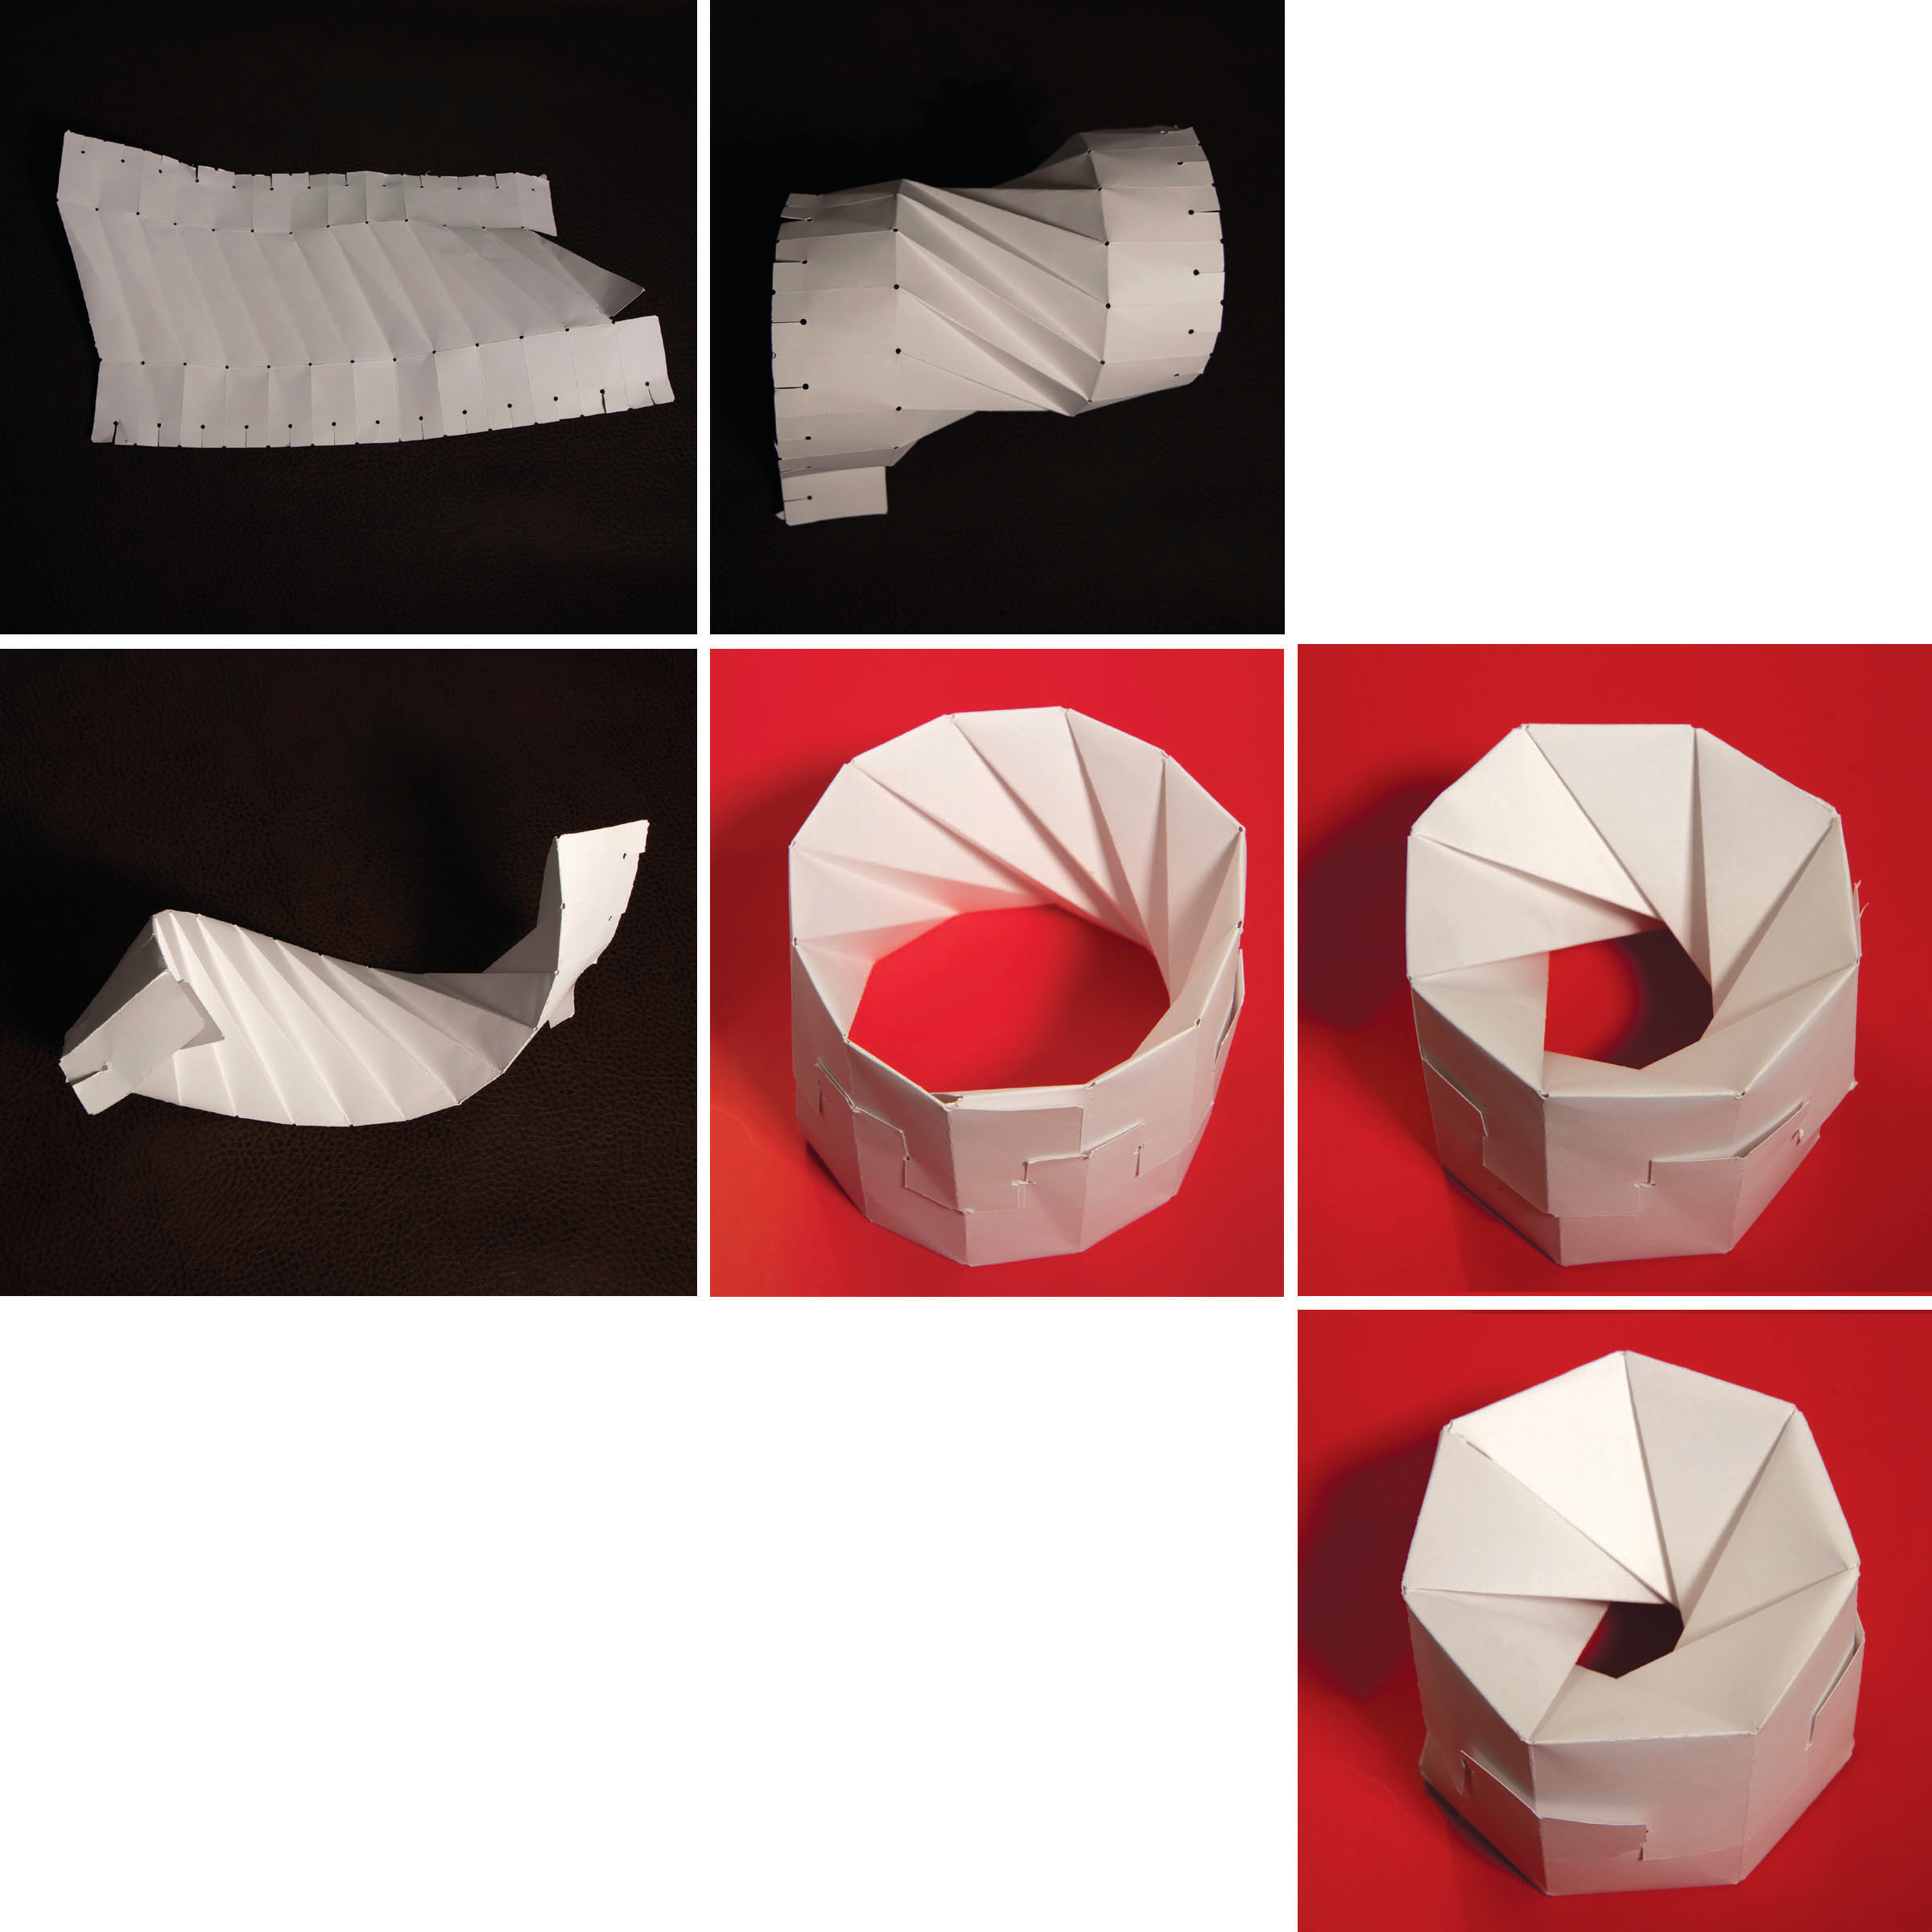
\includegraphics{flat-tori-harris.jpg}}
\end{frame}

\begin{frame}{Pliages en papier hyperbolique (ou Kombucha)}
\protect\hypertarget{pliages-en-papier-hyperbolique-ou-kombucha}{}
\begin{figure}
\centering
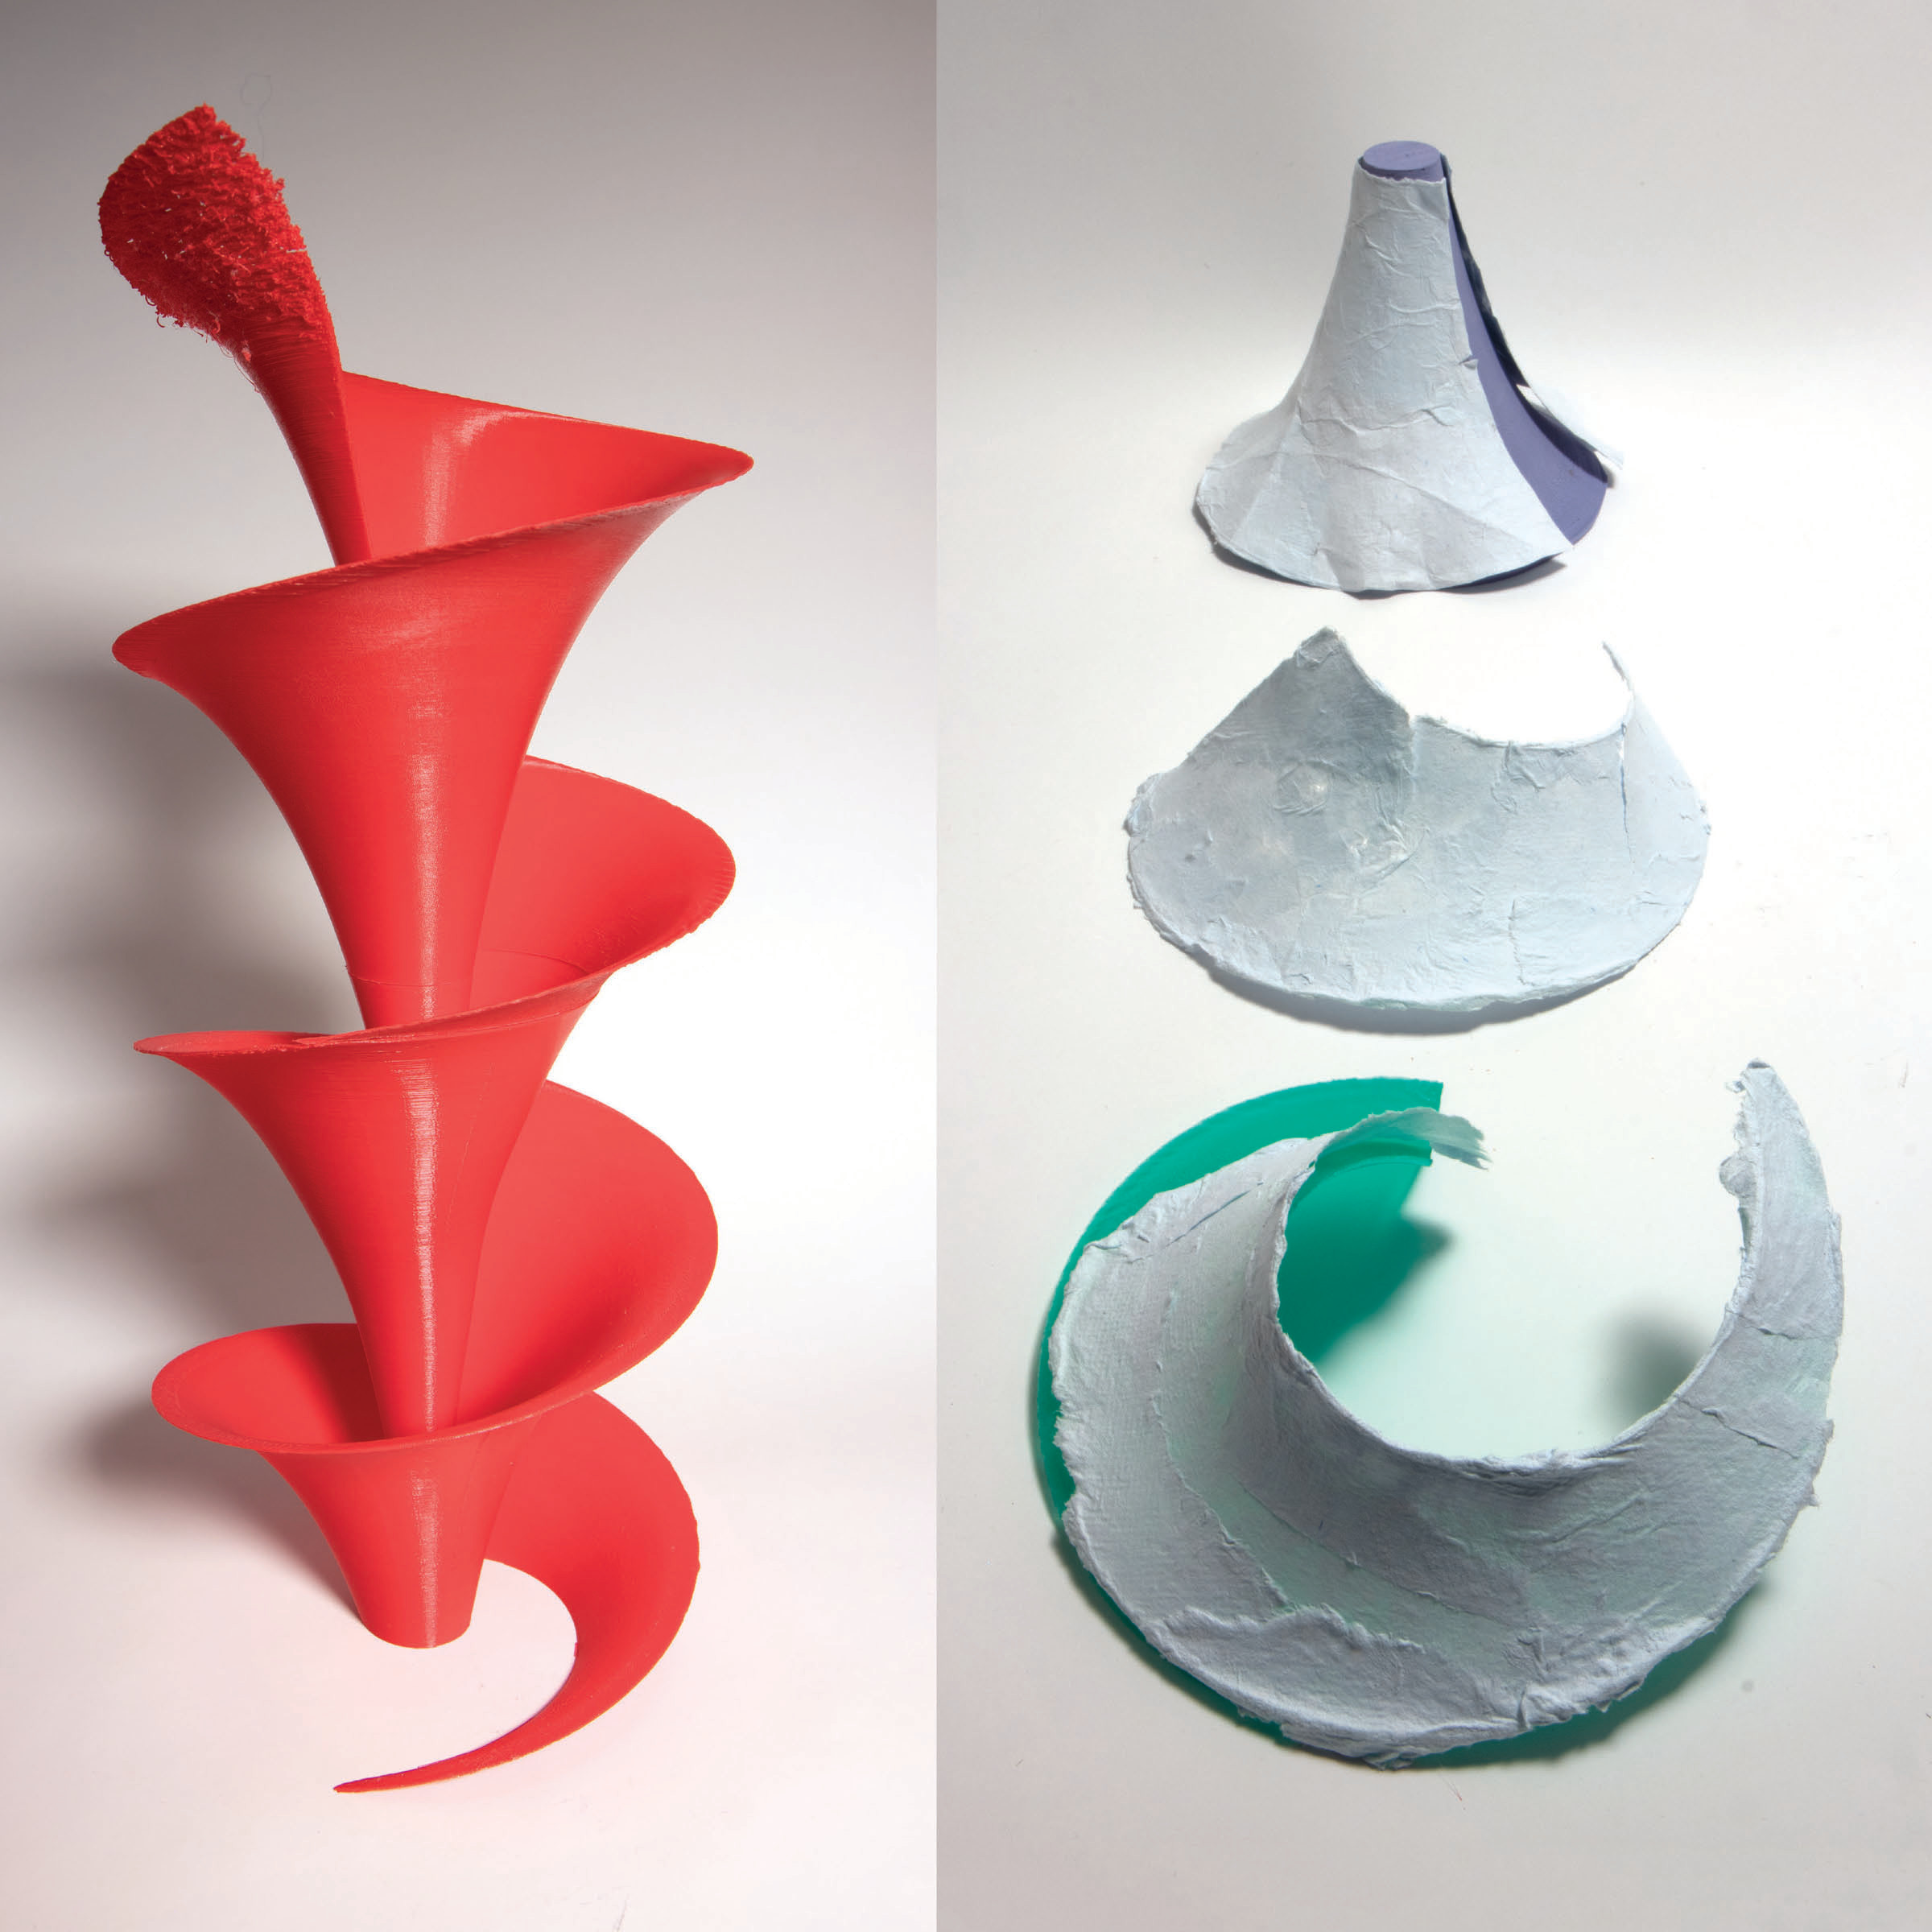
\includegraphics{hyperbolic-paper-harris.jpg}
\caption{Hyperbolic paper from Abrams, Paul, and me.}
\end{figure}
\end{frame}

\begin{frame}{Impression 3D de surfaces algébriques}
\protect\hypertarget{impression-3d-de-surfaces-alguxe9briques}{}
\begin{figure}
\centering
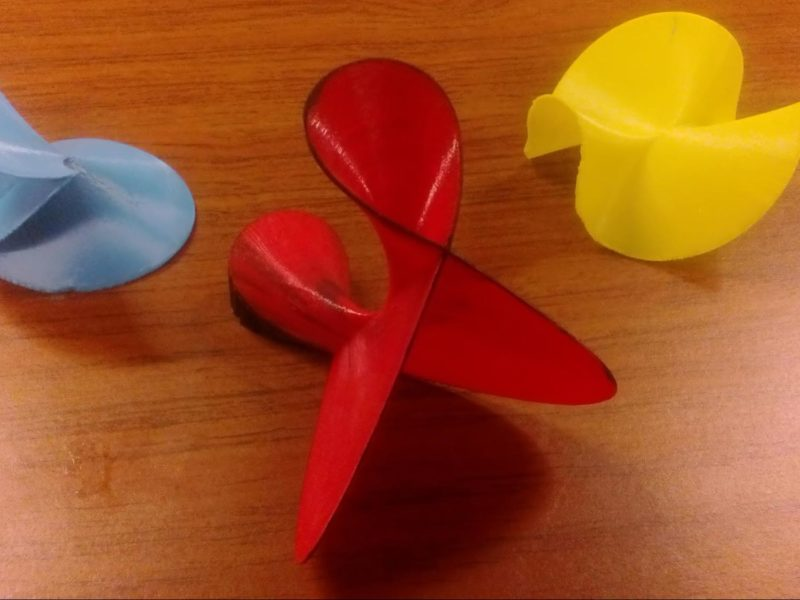
\includegraphics{surfaces-alg.jpg}
\caption{Quelques surfaces algébriques}
\end{figure}
\end{frame}

\begin{frame}
\begin{figure}
\centering
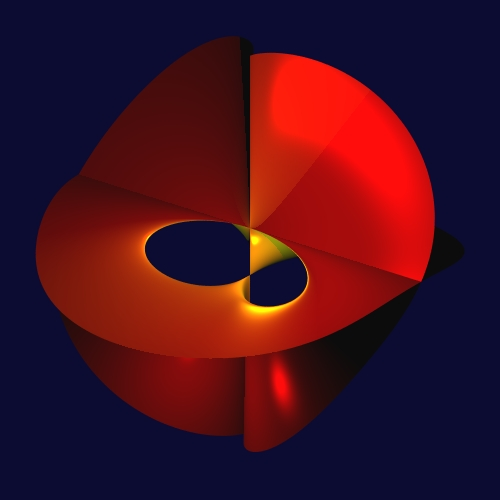
\includegraphics{miau.jpg}
\caption{Miaou par Herwig Hauser}
\end{figure}
\end{frame}

\begin{frame}{Impression 3D d'autres objets mathématiques}
\protect\hypertarget{impression-3d-dautres-objets-mathuxe9matiques}{}
\begin{figure}
\centering
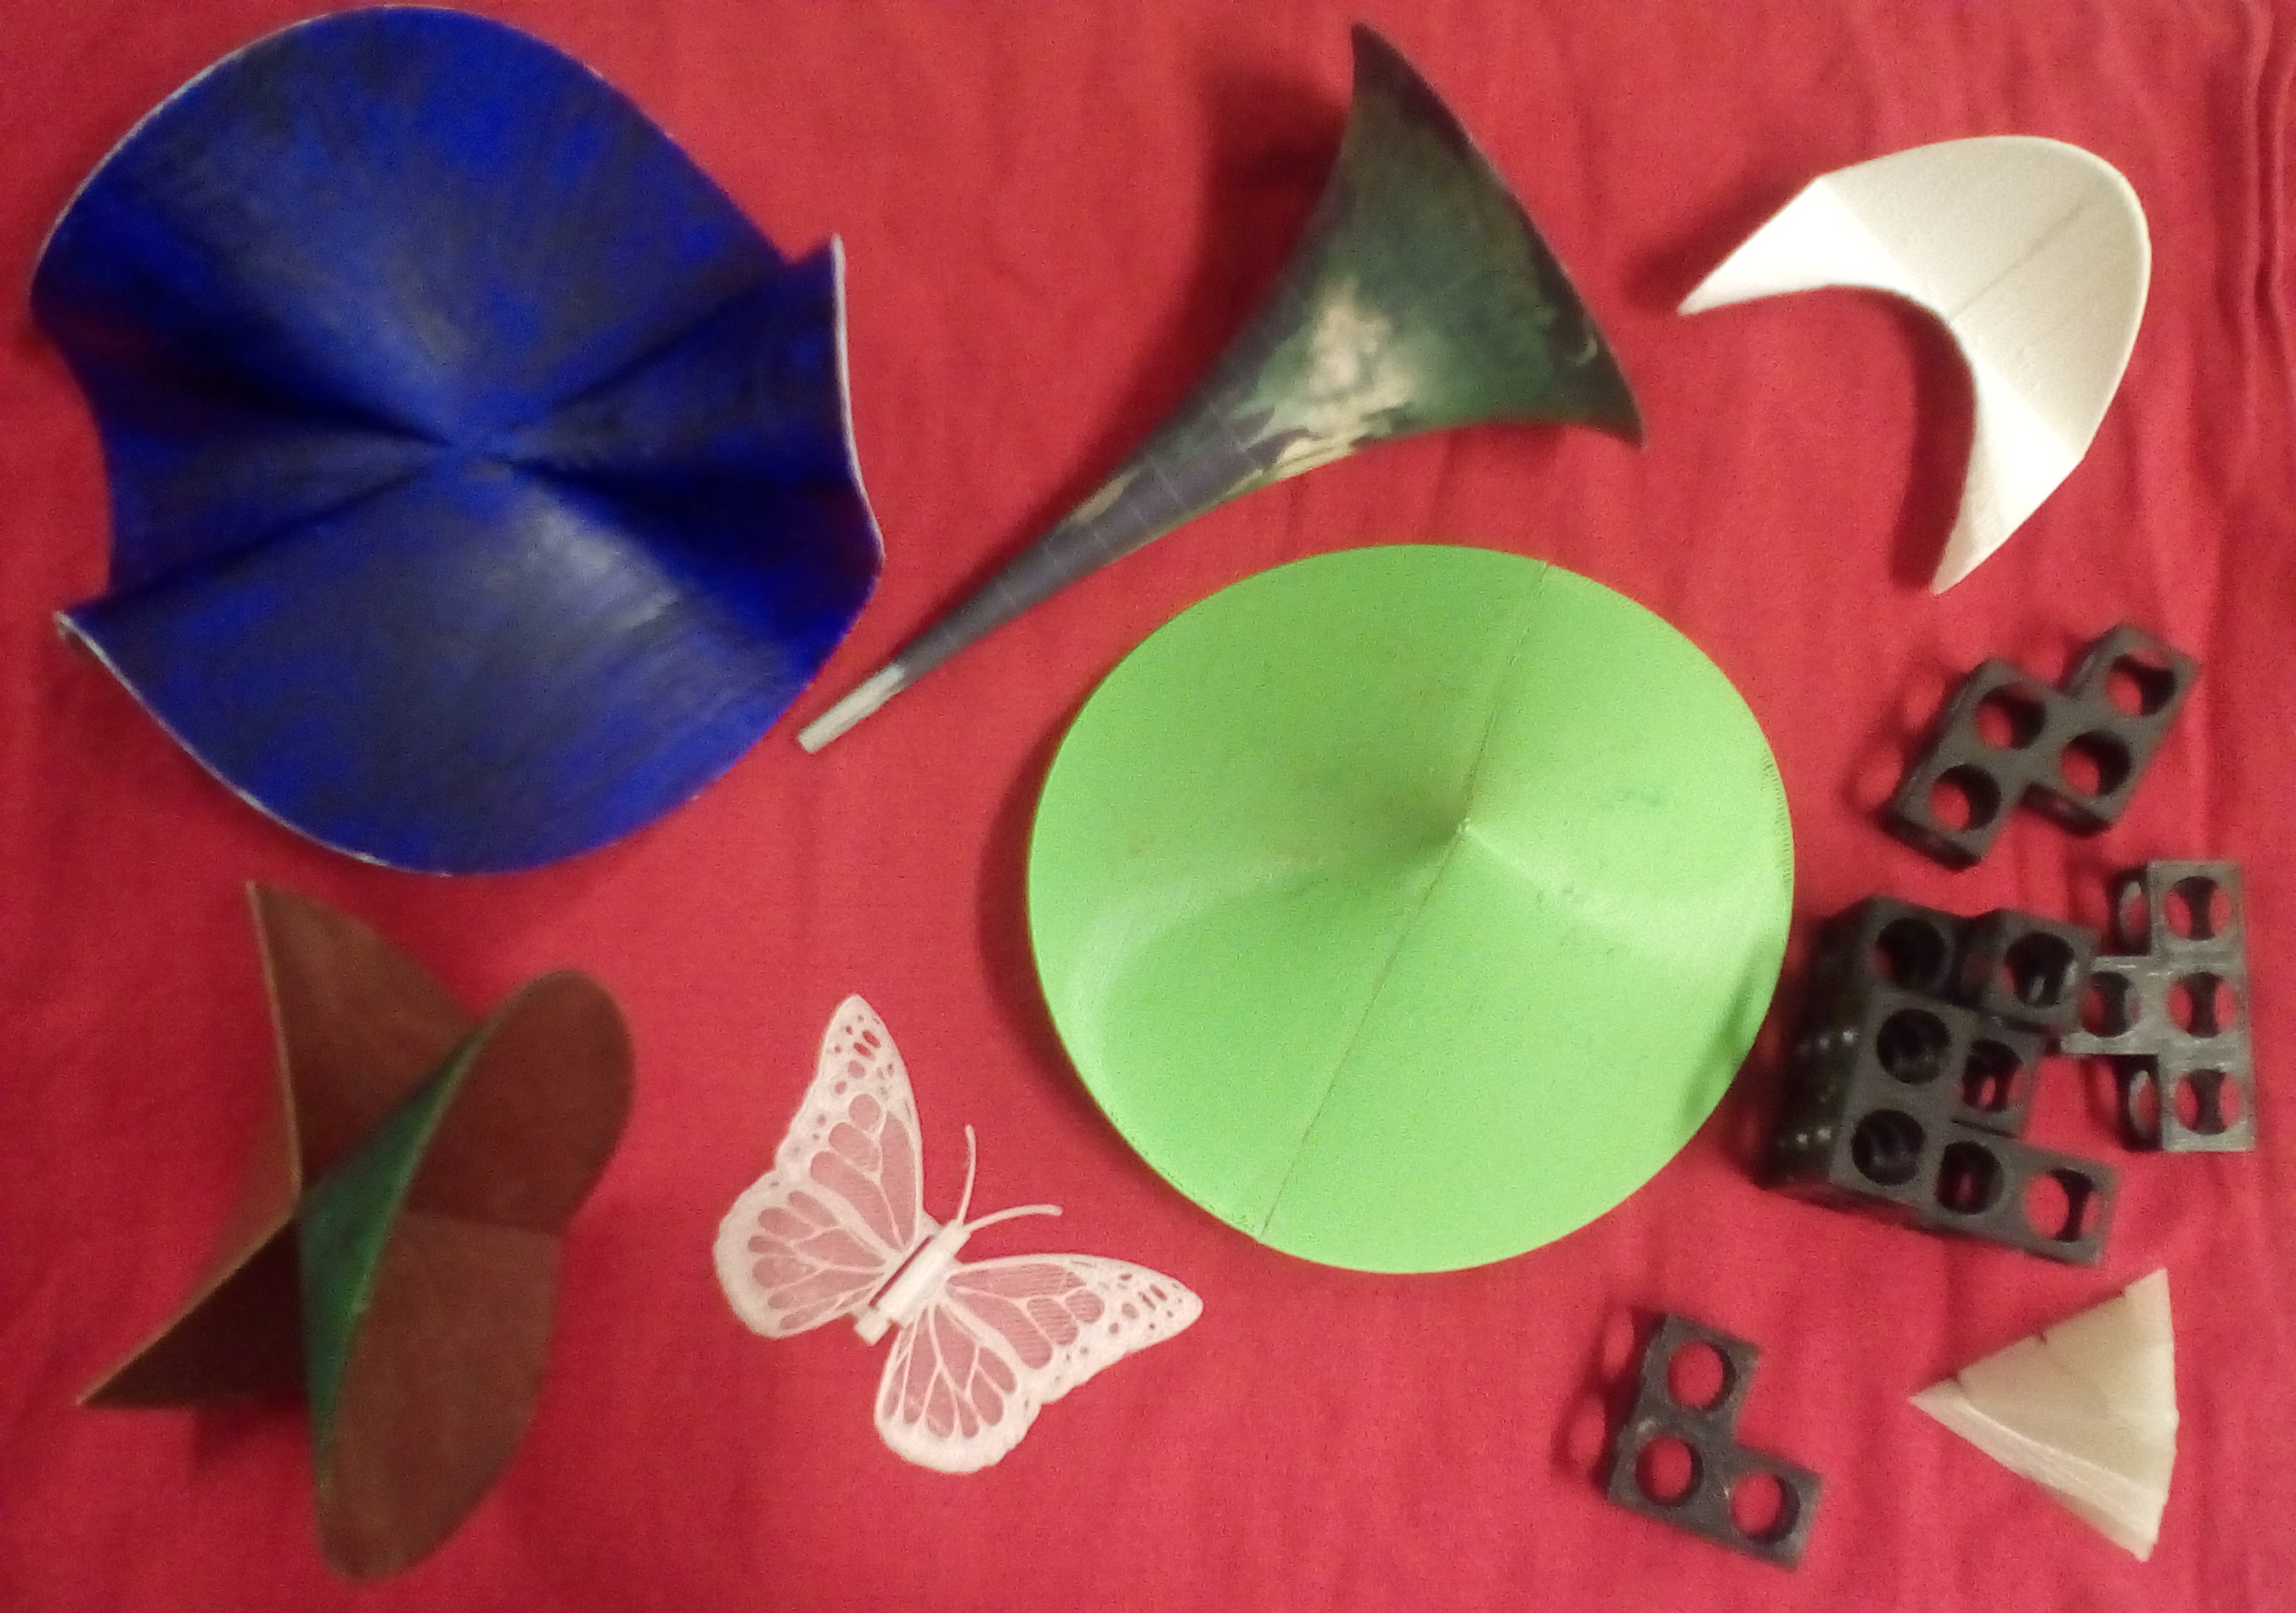
\includegraphics{objets-3D-sur-echarpe-rouge.png}
\caption{objets-3D-sur-echarpe-rouge.png}
\end{figure}
\end{frame}

\begin{frame}{Analyse d'anciens objets en plâtre}
\protect\hypertarget{analyse-danciens-objets-en-pluxe2tre}{}
\begin{figure}
\centering
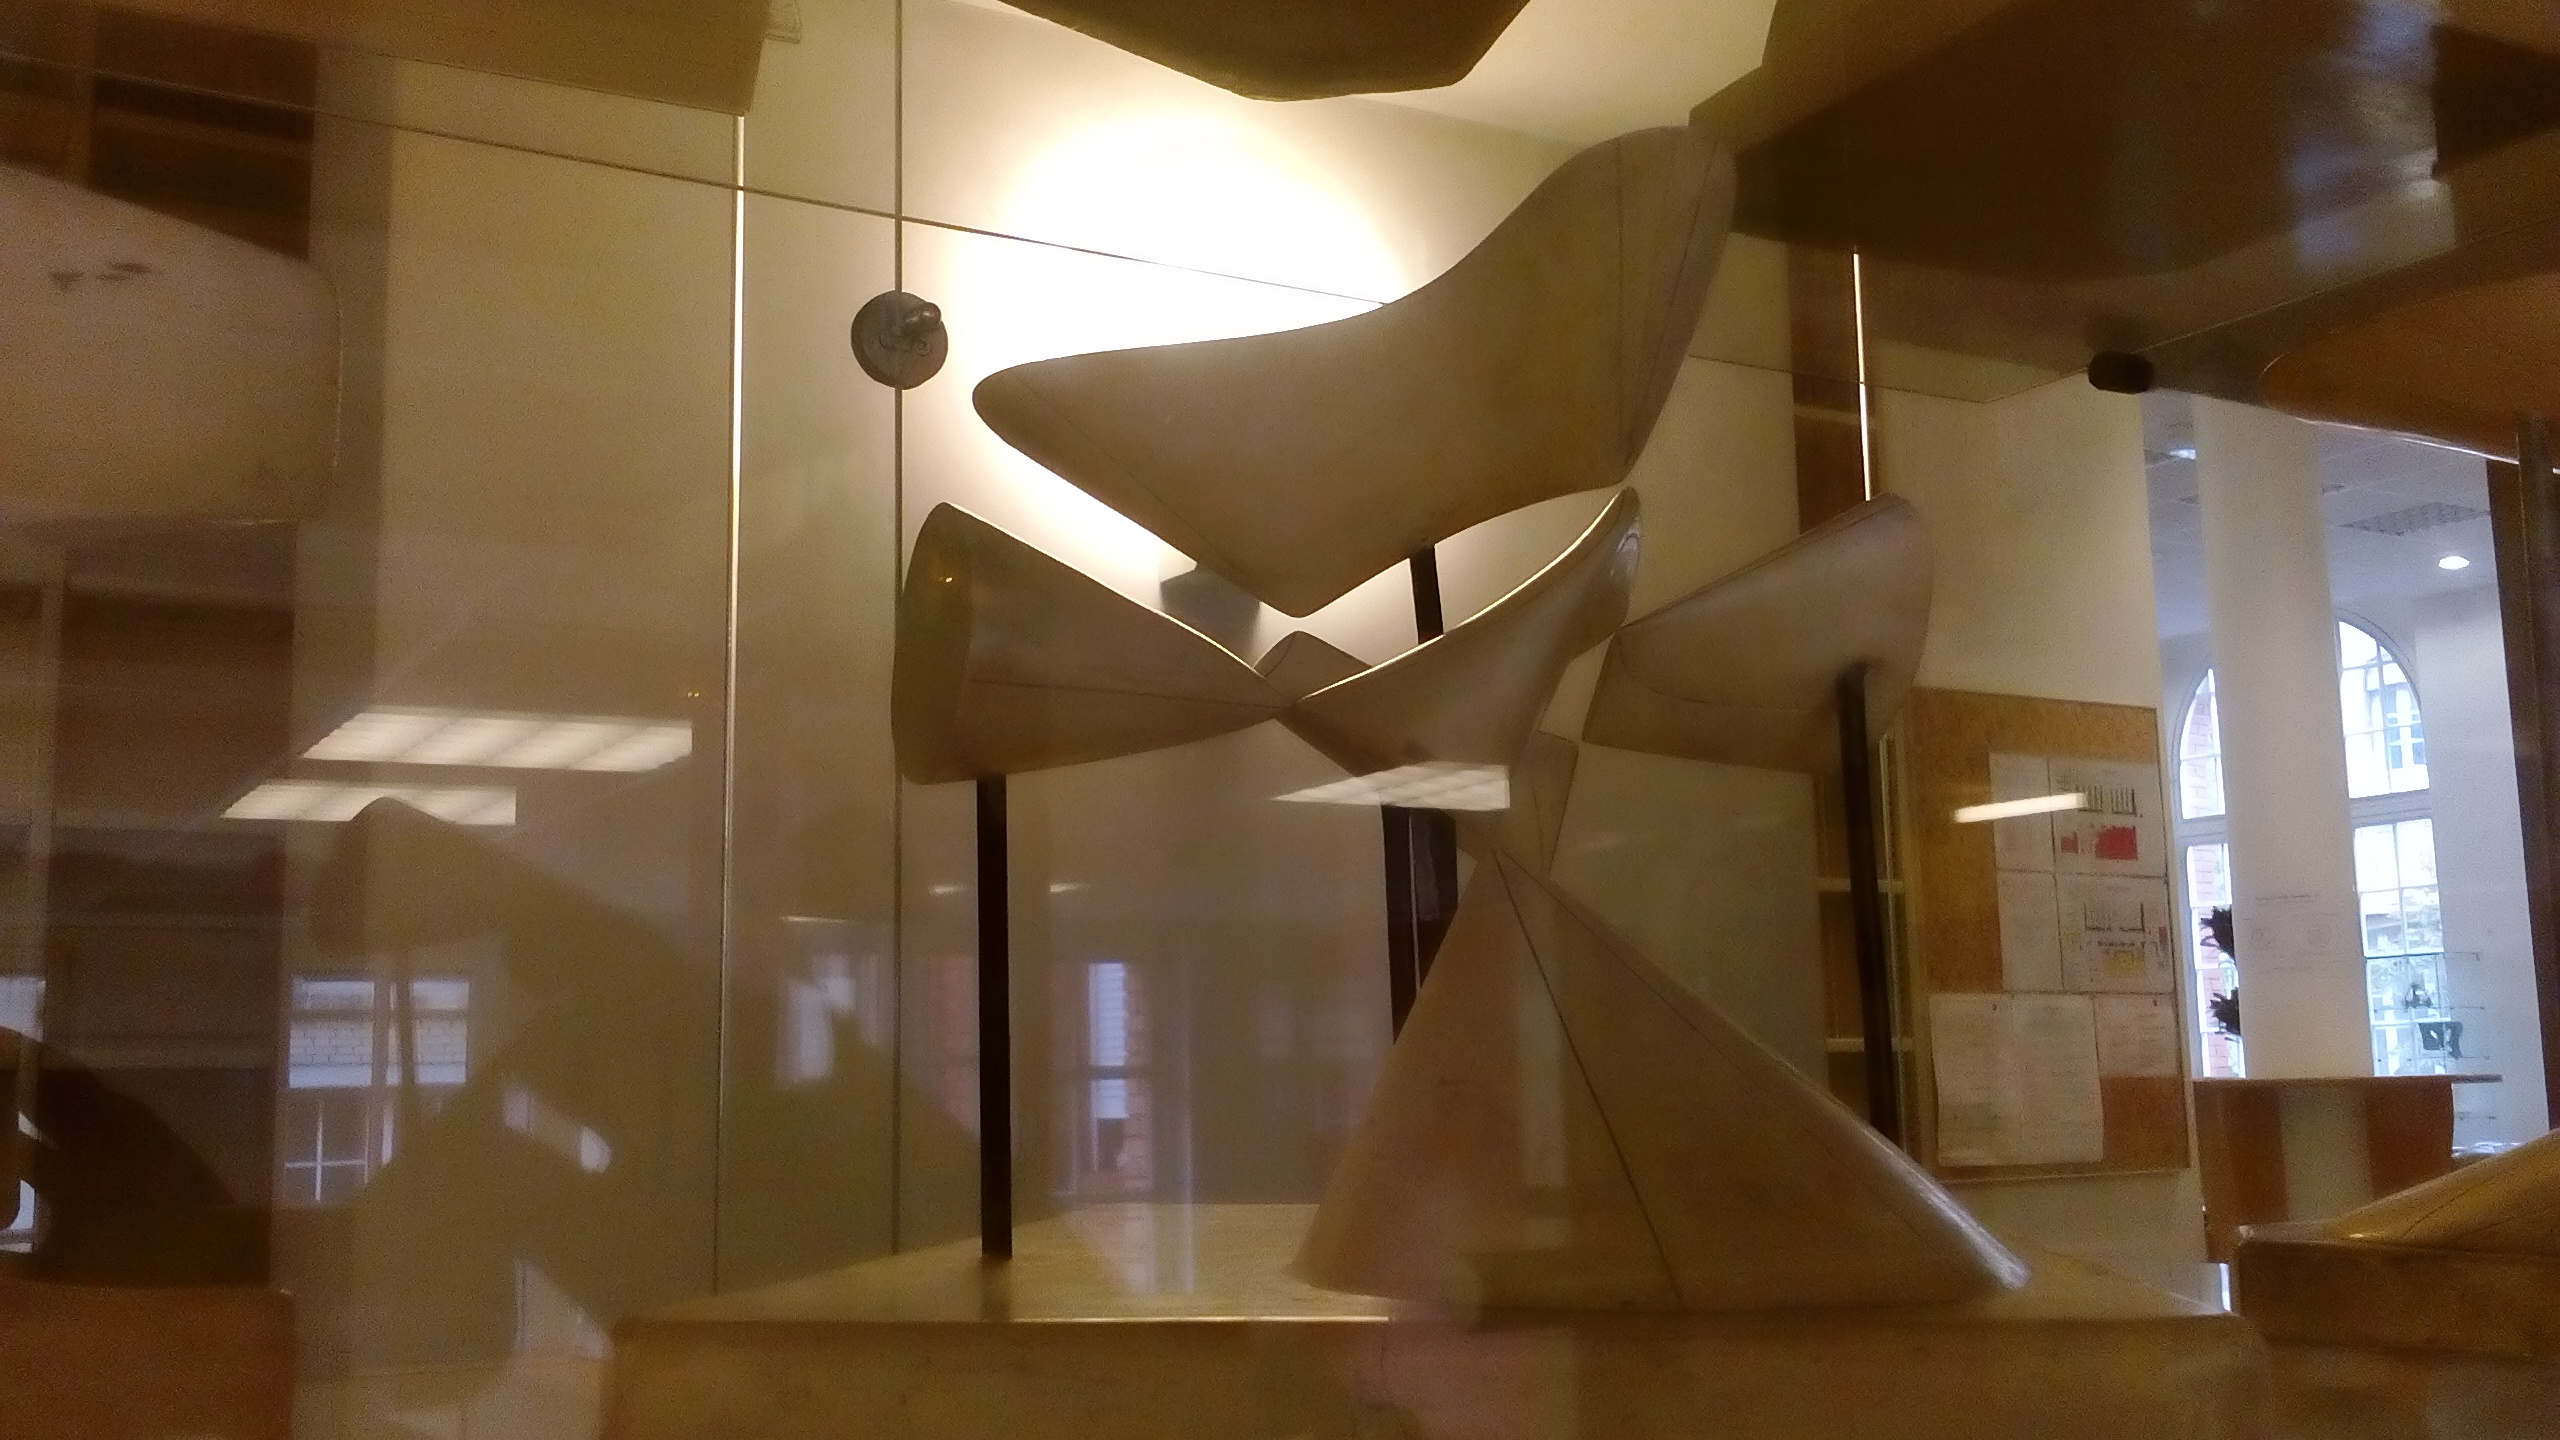
\includegraphics{kummer-platre-a.jpg}
\caption{Surface de Kummer, collections de l'IHP}
\end{figure}
\end{frame}

\hypertarget{ce-que-je-pense-que-je-peut-apporter-dans-gamble}{%
\section{Ce que (je pense que) je peut apporter dans
Gamble}\label{ce-que-je-pense-que-je-peut-apporter-dans-gamble}}

\begin{frame}{En tant que mathématicienne}
\protect\hypertarget{en-tant-que-mathuxe9maticienne}{}
Compétences poussées en:

\begin{itemize}
\tightlist
\item
  géométries 2D et 3D (y compris non-euclidiennes)
\item
  systèmes dynamiques
\end{itemize}

Compétences raisonnables en:

\begin{itemize}
\tightlist
\item
  géométrie algébrique ``à l'ancienne'' (c-à-dire sans schemas)
\item
  géométrie riemannienne
\item
  analyse numérique
\item
  théorie des probabilités
\end{itemize}
\end{frame}

\begin{frame}{En tant que médiatrice scientifique}
\protect\hypertarget{en-tant-que-muxe9diatrice-scientifique}{}
\begin{itemize}
\tightlist
\item
  une facilité à parler de sciences avec\ldots{} tout le monde
\item
  un réseau de contacts en mathématiques qui va bien au-délà de mon
  domaine
\item
  un savoir-faire de ``maker''
\end{itemize}
\end{frame}

\end{document}
